\documentclass[UTF8,twoside,zihao=-4,AutoFakeBold,scheme=chinese,openany]{ctexbook}


% 输入配置文件，例如调用的宏包（公式，插图等）
\input{latex_settings/custom-chinese}

\begin{document}
\pagestyle{empty}
% 中文封面页
\input{chapters/pagetitle-chinese}
% 原创性声明
%% 原创性声明
\begin{center}
  \zihao{3}\textbf{\underline{网络空间安全与信息法学院}本科毕业设计(论文)诚信承诺书}
\end{center}

\zihao{4}
本人郑重承诺：

我向学院呈交的论文《\underline{分布式环境下基于国密的代理重加密设计实现}》，是本人在指导教师的指导下，独立进行研究工作所取得的成果。除文中已经注明引用的内容外，本论文不含任何其他个人或集体已经发表或撰写过的作品成果。对本文的研究做出重要贡献的个人和集体，均已在文中以明确方式标明并致谢。本人完全意识到本声明的法律结果由本人承担。


\vspace{1cm}
\begin{flushright}
年级：\underline{\makebox[3cm]{\hfill 2021\hfill}}\par
专业：\underline{\makebox[3cm]{\hfill 信息安全\hfill}}\par
班级：\underline{\makebox[3cm]{\hfill 40402101\hfill}}\par
承诺人签名：\underline{\makebox[3cm]{\hfill 梁俊勇\hfill}}\par
\vspace{0.3cm}
\underline{2025}年\underline{1}月\underline{1}日
\end{flushright}
\vspace{1cm}
\begin{center}
\zihao{2}\textbf{学位论文版权使用授权书}
\end{center}

本人完全了解重庆邮电大学有权保留、使用学位论文纸质版和电子版的规定，即学校有权向国家有关部门或机构送交论文，允许论文被查阅和借阅等。本人授权重庆邮电大学可以公布本学位论文的全部或部分内容，可编入有关数据库或信息系统进行检索、分析或评价，可以采用影印、缩印、扫描或拷贝等复制手段保存、汇编本学位论文。

（注：保密的学位论文在解密后适用本授权书。）

\vspace{1cm}
\noindent
\begin{tabular}{ll}
学生签名：\underline{\hspace{3cm}} & 指导老师签名：\underline{\hspace{3cm}}\\[0.5cm]
日期：\underline{\hspace{1cm}}年\underline{\hspace{1cm}}月\underline{\hspace{1cm}}日 & 
日期：\underline{\hspace{1cm}}年\underline{\hspace{1cm}}月\underline{\hspace{1cm}}日
\end{tabular}



%% 中文摘要页,开始以罗马字母计页码
\frontmatter
\pagestyle{content}
%% 中文摘要页
\pdfbookmark[0]{摘要}{abstract-zh}
\begin{center}\heiti\sanhao\textbf{
		摘要
	}
\end{center}

为了适应数据要素化背景下数据流通需求场景，
针对分布式环境下多节点参与，数据安全授权变得尤为重要，
本项目提出分布式环境下基于国密的代理重加密算法，
将传统代理重加密中的单代理节点，拆分为多个代理节点，
结合门限代理重加密和国密算法的特点，确保在客户端与中心服务器间、中心服务器与不同节点间、
客户端和不同节点间的数据传输和存储过程中，数据保持完整和隐私性。

与传统的访问控制和权限管理方法相比，
本项目算法具有以下优点：
高强度加密：使用门限代理重加密技术对数据进行高强度加密，保护数据的机密性和隐私性。
分布式架构：采用分布式架构实现对分布式数据的访问控制和授权管理，解决了传统方法在分布式场景下的难题。
自主可控：基于国密算法设计，保证了数据的自主可控性，可以有效地避免数据泄露和信息安全风险。
高效性能：算法实现简单、计算量小，可在现有的计算资源下高效地进行数据安全共享和授权管理。

为了验证所提出系统的有效性和性能，本项目进行了一系列的实验测试。
测试结果表明，该基于国密算法的代理重加密系统在分布式环境中具有优越的加密速度、解密效率和扩展性。

因此，本项目方案为分布式数据的安全传输和存储提供了一个高效且安全的解决方案，
并为区块链环境下隐私计算带来了新的研究视角和实践经验。

\textbf{关键词：}分布式计算；国密算法；代理重加密；数据共享；权限管理
\clearpage

%% 英文摘要页
% 英文摘要页
\pdfbookmark[0]{Abstract}{abstract-en}
\begin{center}\heiti\sanhao\textbf{
		Abstract
	}
\end{center}

In response to the data circulation requirements in the context of data elementization,
data security authorization becomes particularly important in distributed environments with multi-node participation.
This project proposes a distributed proxy re-encryption algorithm based on Chinese cryptographic standards.
The traditional single-proxy node in proxy re-encryption is split into multiple proxy nodes,
combining threshold proxy re-encryption and Chinese cryptographic algorithm characteristics to
ensure data integrity and privacy during data transmission and storage between clients and central servers,
central servers and different nodes,and clients and different nodes.

Compared with traditional access control and permission management methods,
the algorithm in this project has the following advantages:
High-strength encryption:
Uses threshold proxy re-encryption technology to provide high-strength encryption of data,
protecting data confidentiality and privacy.
Distributed architecture:
Implements access control and authorization management for distributed data through a distributed architecture,
solving the challenges faced by traditional methods in distributed scenarios.
Independent control:
Designed based on Chinese cryptographic algorithms,
ensuring data sovereignty and effectively preventing data leakage and information security risks.
High performance:
Simple algorithm implementation with low computational complexity,
enabling efficient data security sharing and authorization management with existing computational resources.

To verify the effectiveness and performance of the proposed system,
this project conducted a series of experimental tests.
The test results show that this proxy re-encryption system based on
Chinese cryptographic algorithms demonstrates superior encryption speed,
decryption efficiency, and scalability in distributed environments.

Therefore, this project provides an efficient and secure solution for distributed data transmission and storage,
bringing new research perspectives and practical experience to privacy computing in blockchain environments.

\textbf{Keywords:} Distributed Computing; Chinese Cryptographic Algorithm; Proxy Re-encryption; Data Sharing

\newpage\quad %加一页，使得目录第一页的页眉为 目录
\clearpage


%% 目录
\pagestyle{headings}
\tableofcontents
% % \thispagestyle{MyStyle}
\let\cleardoublepage\clearpage %latex消除空白页

% ===============================
% 开始章节写作,显示特定页眉页脚
\mainmatter
\pagestyle{plain}
% 第1-7章
\chapter{引言}

\section{研究背景和意义}

随着数字经济的快速发展，数据要素化已成为推动经济社会发展的重要驱动力。
在分布式环境下，数据的安全流通和共享变得愈发重要，
尤其是在涉及多个参与节点的场景中，如何保证数据传输和存储过程的安全性成为亟待解决的关键问题。

如何结合分布式技术完成数据的安全共享一直是热门研究方向，
自从2008年Nakamoto
\cite{nakamoto2008bitcoin}
（中本聪）发表了一篇《比特币：一种点对点的电子现金系统》后，
吸引了无数来自不同学术领域的学者的关注。

当前，传统的数据安全授权方案在分布式环境下面临诸多挑战：
首先，单一的授权节点容易成为系统安全的薄弱环节；
其次，现有的授权机制难以满足分布式环境下多方协同的需求；
最后，在确保数据安全的同时如何保持系统效率，也是一个重要问题。

本课题的研究对推动数据要素安全流通具有重要的理论和实践意义。
在理论层面，本研究将门限密码学与代理重加密技术相结合，
拓展了传统代理重加密的应用场景。在实践层面，本研究提出的基于国密算法的分布式代理重加密方案，
为解决分布式环境下的数据安全授权问题提供了可行的技术路径。

\section{国内外研究现状}

\subsection{国外研究现状}

在国外，代理重加密技术的研究始于Blaze\cite{blaze1998divertible}等人1998年提出的概念。
近年来，随着分布式系统的普及，国际学术界对分布式环境下的数据安全授权展开了深入研究。主要包括：

1）基于属性的代理重加密方案，实现了更细粒度的访问控制

2）门限代理重加密技术，提高了系统的容错性和可靠性

3）基于格密码的代理重加密方案，为抵抗量子计算攻击提供了可能

\subsection{国内研究现状}

国内在数据安全授权领域的研究主要集中在以下方面：

1）国密算法在代理重加密中的应用研究

2）基于区块链的分布式授权机制研究

3）面向特定领域的数据安全共享方案研究

然而，目前的研究仍存在一些不足，如计算效率有待提高、安全性证明不够完备等问题。

\section{主要内容和工作安排}

本文共分为五章，具体安排如下：

第1章为引言，介绍研究背景、意义及国内外研究现状。

第2章为理论基础，阐述代理重加密、门限密码和国密算法的基本原理。

第3章为系统设计，详细描述分布式环境下基于国密的代理重加密方案。

第4章为实验验证，通过多组对比实验验证系统的性能和安全性。

第5章为总结与展望，总结研究成果并提出未来的研究方向。

本研究预期在保证数据安全性的同时，实现高效的分布式数据授权管理，为解决数据要素化背景下的数据安全流通问题提供新的技术方案。

\chapter{理论基础}

\section{代理重加密}

代理重加密是一种特殊的公钥加密技术，允许代理为第三方重加密消息，
而不需要知道消息的具体内容。
这项技术使得原始加密数据的所有者可以授权代理为第三方重新加密其数据，
而不必将原始数据或解密密钥透露给代理，从而保证了数据安全性和保密性。

\subsection{基本原理}

在代理重加密系统中，通常涉及三个角色：数据拥有者(Alice)、数据接收者(Bob)和代理服务器。其工作流程如下：

\begin{enumerate}
	\item Alice首先使用自己的公钥对数据M进行加密，产生密文C
	\item 当Alice希望Bob能够访问其加密数据时，她会创建一个重加密密钥rk，并将其提供给代理服务器
	\item 代理服务器使用重加密密钥rk将Alice的加密数据C转化为重加密密文C'
	\item Bob使用自己的私钥对重加密密文C'进行解密，得到原始数据M
\end{enumerate}

在这个过程中，代理服务器既不能访问原始数据，也不能访问解密密钥，从而保证了数据的安全性。

\section{门限密码}

\section{Shamir密码共享方案}

Shamir密码共享方案其核心思想是通过多项式插值来达到一个目的，由Adi Shamir
\cite{Shamir1979How}
在1979年提出。其定义如下：

$(t,n)$-Shamir是一种方法，使得一个秘密$S$可以被分割为$n$个片段$\{s_1,\ldots,s_n\}$，
这样只有当至少$t$个片段（其中$t \leq n$）集合在一起时，才能恢复原始的秘密$S$。
如果只有$t-1$个或更少的片段，则无法获得任何关于秘密的信息。
这种属性称为$(t,n)$阈值方案，其中$t$（也即$threshold$）是必要的片段数量，
$n$是总片段数量。Shamir密码共享方案的原理基于数学中的多项式插值，
尤其是Lagrange插值。以下是其工作原理：

\begin{enumerate}
	\item 选择一个整数$t$，表示需要的最少片段数来恢复秘密。
	\item 为秘密构造一个$t-1$次多项式$f(x)$，其中$f(0)=S$是要分享的秘密：
	      \[f(x) = a_0 + a_1x + a_2x^2 + \cdots + a_{t-1}x^{t-1}\]
	      其中$a_0 = S$，其他系数$a_1,\ldots,a_{t-1}$随机选择。
	\item 为每个参与者选择一个不同的$x$值，并计算相应的$f(x)$。每个$(x,f(x))$对都是一个秘密片段。
	\item 当要恢复秘密时，只需要任意$t$个$(x,f(x))$对，并使用Lagrange插值来恢复$f(0)$，即原始的秘密$S$。
\end{enumerate}

% FIX: 修改例子的数据
举例说明：假设我们有一个秘密数字$S=42$，我们希望将其分割成3个片段，
但只需要2个片段就可以恢复它（即$t=2,n=3$）：

选择一个一次多项式（因为$t-1=1$）:
\[f(x) = a_0 + a_1x\]

假设我们选择$a_1=17$，那么多项式就是：
\[f(x) = 42 + 17x\]

为每个参与者选择一个$x$值并计算$f(x)$：
\[f(1) = 42 + 17(1) = 59\]
\[f(2) = 42 + 17(2) = 76\]
\[f(3) = 42 + 17(3) = 93\]

每个参与者分别得到一个片段：$(1,59)$，$(2,76)$和$(3,93)$。
要恢复秘密，我们可以选择其中任意两个片段。
假设我们选择$(1,59)$和$(2,76)$，使用Lagrange插值可以计算出$f(0)=42$，从而恢复秘密。

具体的Lagrange插值公式为：
\[f(x) = \sum_{i=1}^t y_i \prod_{j=1,j\neq i}^t \frac{x-x_j}{x_i-x_j}\]

在这个例子中，使用$(1,59)$和$(2,76)$进行插值：
\[f(0) = 59\cdot\frac{0-2}{1-2} + 76\cdot\frac{0-1}{2-1} = 59\cdot(-2) + 76\cdot(-1) = -118 + (-76) = 42\]

这就恢复出了原始的秘密值42。这个例子展示了Shamir密码共享方案的基本原理和实际应用。

该方案的安全性基于：
\begin{itemize}
	\item 任意$t-1$个或更少的点无法确定一个$t-1$次多项式
	\item 多项式的系数（除$a_0$外）是随机选择的
	\item 在有限域上进行运算可以进一步增强安全性
\end{itemize}

\section{非对称/公钥密码算法}
% FIX: 不应该直接复制wiki，需要改写
公开密钥密码学（英语：Public-key cryptography）
也称非对称式密码学（英语：Asymmetric cryptography）
是密码学的一种算法，它需要两个密钥，一个是公开密钥，
另一个是私有密钥；公钥用作加密，私钥则用作解密。
使用公钥把明文加密后所得的密文，只能用相对应的私钥才能解密并得到原本的明文，
最初用来加密的公钥不能用作解密。由于加密和解密需要两个不同的密钥，故被称为非对称加密；

\subsection{基于大因数分解}
代表算法：RSA

这类算法的安全性基于大整数分解问题的难度。
RSA算法的安全性依赖于将两个大质数的乘积进行因式分解的计算复杂度。
目前已知的最高效算法仍需要超多项式时间，这保证了在足够大的密钥长度下的安全性。
RSA广泛应用于数字签名、密钥交换和数据加密等场景。

\subsection{基于离散对数}
代表算法：DSA、Diffie-Hellman

这类算法的安全性基于在有限域中计算离散对数的难度。
DSA（数字签名算法）主要用于生成数字签名，而Diffie-Hellman则是一种密钥交换协议，
允许通信双方在不安全的通信信道上建立共享密钥。这些算法在安全通信和身份验证中扮演重要角色。

\subsection{基于椭圆曲线}
代表算法：ECDSA、ECDH、SM2

椭圆曲线密码学利用定义在有限域上的椭圆曲线数学性质
。与传统公钥密码相比，椭圆曲线密码在相同安全水平下需要更短的密钥长度，
提供了更高的计算效率和带宽节约。SM2是中国国家密码算法标准，
是基于椭圆曲线的公钥密码算法，支持数字签名、密钥交换和数据加密功能。

\section{杂凑算法}
杂凑算法（也称散列算法或哈希算法）是将任意长度的输入数据转换为固定长度输出的单向函数。

理想的杂凑算法应满足以下特性：
\begin{itemize}
	\item 单向性：由杂凑值无法逆向推导出原始输入
	\item 抗碰撞性：难以找到具有相同杂凑值的两个不同输入
	\item 雪崩效应：输入的微小变化会导致输出的显著变化
\end{itemize}

常见的杂凑算法包括：
\begin{itemize}
	\item MD5：输出128位杂凑值，现已被证明存在安全缺陷
	\item SHA家族：包括SHA-1（160位）、SHA-2（224/256/384/512位）和SHA-3系列
	\item SM3：中国商用密码杂凑算法标准，输出256位杂凑值
\end{itemize}

杂凑算法广泛应用于数字签名、消息认证码、数据完整性校验和密码存储等场景。

\section{对称密码算法}
对称密码算法（英语：Symmetric-key algorithm）使用相同的密钥进行加密和解密操作。
与非对称加密相比，对称加密计算效率更高，
但密钥分发和管理存在挑战。对称密码主要分为分组密码和流密码两大类。

\subsection{分组密码算法}
分组密码将明文分割成固定长度的数据块，然后对每个块进行加密处理。主要特点包括：

\begin{itemize}
	\item 以固定大小的块为单位进行加密
	\item 相同的明文块在相同密钥下产生相同的密文块
	\item 需要配合工作模式使用（如ECB、CBC、CTR等）以处理超出块大小的数据
\end{itemize}

代表算法：
\begin{itemize}
	\item DES：56位密钥，64位分组，现已不再安全
	\item 3DES：基于DES的三重加密，提高安全性但速度较慢
	\item AES：分组大小128位，支持128/192/256位密钥长度
	\item SM4：中国商用分组密码标准，128位分组和密钥长度
\end{itemize}

\subsection{流密码算法}
流密码算法产生一个伪随机密钥流，通过与明文逐位（通常是按位异或）组合来生成密文。主要特点：

\begin{itemize}
	\item 逐位或逐字节处理数据，无需分组
	\item 加密和解密操作相同
	\item 适合实时性要求高或硬件资源受限的场景
\end{itemize}

代表算法：
\begin{itemize}
	\item RC4：曾广泛应用于SSL/TLS、WEP等协议，但现已被证明存在多种安全问题
	\item ChaCha20：现代高性能流密码，被用于TLS 1.3和许多安全通信场景
	\item ZUC：中国商用流密码标准，用于4G/5G移动通信安全
\end{itemize}

流密码算法通常具有更高的加密速度和更低的实现复杂度，
特别适合对吞吐量要求高或资源受限的环境，如无线通信和嵌入式系统。

\section{国密算法}

国密算法是我国自主研发的一系列密码算法标准，主要包括SM2、SM3和SM4等。

\subsection{SM2公钥密码算法}

SM2算法是我国基于椭圆曲线密码体制自主研发的公钥密码算法，包含以下三个主要功能：

\begin{itemize}
	\item SM2-1：数字签名算法
	\item SM2-2：密钥交换协议
	\item SM2-3：公钥加密算法
\end{itemize}

相比于传统RSA签名算法，SM2的主要优势在于：
\begin{itemize}
	\item 安全性基础：SM2基于椭圆曲线上的离散对数问题(ECDLP)，而RSA基于整数分解问题(IFP)
	\item 密钥长度：SM2可以用更短的密钥实现与RSA相同的安全强度\cite{nist800-57r5}
	\item 计算效率：在同等安全级别下，SM2的椭圆曲线运算比RSA的大整数模幂运算更高效\cite{hankerson2006guide}
\end{itemize}

% 或者也可以将两个引用合并成一个：
这些优势已在多项研究中得到证实\cite{nist800-57r5,hankerson2006guide}。

\subsection{SM3密码杂凑算法}

SM3哈希算法是密码体系的重要组成部分，是一种将任意长度的消息$M$映射为定长字符串$H(M)$的单向散列函数，
$H(M)$称为$M$的消息摘要。我国基于对SHA-256中的压缩函数进行自主研发并取得重大突破，
国产哈希算法SM3随之诞生。与SHA-256相似，SM3算法同样适用于数字签名、消息认证及随机数生成等场景，
且其安全性略高于SHA-256，国家密码管理局规定SM2算法中的哈希算法为SM3。\cite{SM3StandardGroup2013}

SM3算法对长度为$l$比特的消息$M$，经过填充和迭代压缩，最终输出一个256比特的杂凑值。算法主要包含以下步骤：

\subsubsection{填充过程}
设有长度为$l$比特的消息$M$：
\begin{enumerate}
	\item 首先将比特"1"添加至消息$M$末尾
	\item 添加$k$个"0"，其中$k$是满足公式$(l + 1 + k) \bmod 512 = 448$的最小非负整数
	\item 添加一个64位比特串，表示$l$的值
	\item 填充后的消息$M$比特长度为512的倍数
\end{enumerate}

\subsubsection{迭代压缩过程}
分为以下两个主要步骤：

1. 消息分块与扩展：
\begin{itemize}
	\item 将填充好的消息$M$按每512比特分成$n$个组，其中$M = M^{(1)} || M^{(2)} || ... || M^{(n)}$
	\item 将上述分组按消息扩展算法扩展成132个消息字$W_j$，用于压缩函数$CF$
\end{itemize}

2. 压缩与输出：
\begin{itemize}
	\item 对分组后的消息$M$进行$n$次迭代压缩
	\item $V_i = CF(V_{i-1}, M^{(i)})$，其中$i = 1,2,...,n$
	\item $CF$为压缩函数，通过最终的迭代值得到一个256比特的杂凑值
\end{itemize}



\subsection{SM4分组密码算法}

SM4是一种对称密钥分组密码算法，是SMS4算法的标准化版本。其主要特征如下：

\subsubsection{基本参数}
\begin{itemize}
	\item 分组大小：128位
	\item 密钥长度：128位
	\item 加密轮数：32轮
\end{itemize}

\subsubsection{算法结构}
\begin{itemize}
	\item 采用"置换-置换"(SP)网络结构，区别于传统的"置换-替代"(SPN)结构
	\item 包含非线性变换函数（S盒）：将4字节输入转换为4字节输出
	\item 线性变换：用于增强加密强度
	\item 轮函数：每轮使用$F$函数处理数据块和轮密钥
\end{itemize}

\subsubsection{密钥处理}
\begin{itemize}
	\item 密钥扩展：从128位主密钥生成32个轮密钥
	\item 轮密钥加：通过异或运算将轮密钥与数据块结合
\end{itemize}

\subsubsection{工作模式}
SM4支持多种标准工作模式：
\begin{itemize}
	\item ECB（电子密码本模式）
	\item CBC（密码分组链接模式）
	\item CTR（计数器模式）
	\item 其他标准分组密码工作模式
\end{itemize}

\subsection{混合加密机制}

\subsubsection{基本原理}
由于公钥密码算法是基于复杂的代数计算，其计算效率远低于对称密码算法。
因此，在需要加密大量数据时，直接使用公钥密码进行加密并不是最优选择。
为解决这一问题，现代密码学中普遍采用KEM/DEM混合加密机制：

\begin{itemize}
	\item KEM (Key-Encapsulation Mechanism)：密钥封装机制
	\item DEM (Data-Encapsulation Mechanism)：数据封装机制
\end{itemize}

\subsubsection{工作机制}
KEM/DEM混合加密方案的工作流程如下：

1. 数据加密过程：
\begin{itemize}
	\item DEM使用对称加密算法加密原始数据
	\item 随机生成用于对称加密的会话密钥
	\item KEM使用公钥加密算法对会话密钥进行加密
\end{itemize}

2. 数据解密过程：
\begin{itemize}
	\item 接收方首先使用私钥解密得到会话密钥
	\item 使用恢复的会话密钥解密获得原始数据
\end{itemize}

\subsubsection{优势特点}
KEM/DEM混合加密机制具有以下优势：

\begin{enumerate}
	\item 效率提升
	      \begin{itemize}
		      \item 大量数据使用高效的对称加密
		      \item 仅对短小的会话密钥使用公钥加密
		      \item 显著提高整体加解密效率
	      \end{itemize}

	\item 安全性保障
	      \begin{itemize}
		      \item 结合对称加密和非对称加密的安全优势
		      \item 即使会话密钥泄露也不影响其他通信场景
		      \item 支持前向安全性
	      \end{itemize}

	\item 通信优化
	      \begin{itemize}
		      \item 减少加密数据的传输量
		      \item 降低网络带宽占用
		      \item 提高通信效率
	      \end{itemize}
\end{enumerate}

\subsubsection{应用场景}
混合加密机制在以下场景中具有广泛应用：

\begin{itemize}
	\item 安全通信协议（如TLS/SSL）
	\item 数据加密传输
	\item 文件加密存储
	\item 密钥交换协议
\end{itemize}

\subsubsection{具体实现}
在实践中，KEM/DEM 混合加密机制通常采用以下算法组合：
1. KEM (密钥封装机制) 实现选择：
\begin{itemize}
	\item 基于椭圆曲线的算法：SM2、ECIES、ECDH 等
	\item 基于整数分解的算法：RSA-OAEP、RSA-KEM 等
	\item 基于格的后量子算法：CRYSTALS-Kyber、NTRU 等
	\item 基于配对的算法：IBE-KEM (基于身份的加密)
\end{itemize}

2. DEM (数据封装机制) 实现选择：
\begin{itemize}
	\item 分组密码及其工作模式：SM4-GCM、AES-GCM、ChaCha20-Poly1305 等
	\item 结合 AEAD (认证加密与关联数据) 模式确保机密性和完整性
	\item 针对高性能需求的流密码或轻量级分组密码：SNOW、AEGIS 等
\end{itemize}

\section{本章小结}

本章介绍了分布式环境下基于国密的代理重加密系统所需的核心理论基础，
包括代理重加密技术、门限密码学和国密算法。
这些理论为系统的设计和实现提供了必要的技术支撑，
确保了系统的安全性、可靠性和高效性。

\chapter{系统设计与实现方案}
\section{总体设计}
分布式环境下数据安全共享已成为数字经济发展的关键挑战与机遇。随着云计算、区块链、
物联网等技术的广泛应用，数据作为核心生产要素的价值日益凸显，
然而数据安全流通与共享面临诸多技术障碍。传统密码学体系在分布式场景下暴露出密钥管理复杂、
授权控制僵化、计算效率有限等问题，无法满足现代数据共享生态的灵活性与安全性需求。
本系统通过创新性地结合门限密码学与代理重加密技术，构建了一种适应分布式环境的安全数据共享架构，
实现了数据价值流动与隐私保护的平衡。

本方案的核心技术创新在于将门限密码学的分布式信任机制与代理重加密的授权转换能力有机融合，
形成了一个既保障数据机密性又支持灵活授权的安全框架。在该框架中，
数据所有者无需直接向被授权方透露原始密钥，而是通过可信代理节点集合执行密文转换，
实现了"数据不动、密钥不共享"的安全共享范式。特别地，
本系统采用国家密码管理局认证的商用密码算法（即"国密算法"）作为基础密码组件，
不仅确保了系统的安全强度，还满足了国内关键信息基础设施的合规要求。
国密算法（如SM2、SM4、SM3等）在密码学理论基础和工程实现上均已成熟，
其安全性已经过充分论证和广泛验证，为系统提供了坚实的安全基础。

本系统的分布式架构设计充分考虑了现代数据生态的复杂性和动态性，通过多节点协同工作机制，
有效规避了中心化系统的单点故障风险和性能瓶颈问题。系统中的代理节点群采用分布式共识协议进行协调，
每个节点仅持有部分重加密密钥，任何单一节点的妥协都不会危及整体系统安全。
这种设计不仅提高了系统的容错性和可用性，还通过负载均衡和并行处理能力，
实现了处理大规模并发请求的能力，满足企业级应用和大数据环境的性能要求。
分布式架构还具备良好的可扩展性，系统可根据实际需求动态调整节点数量和分布，
适应不同规模和复杂度的应用场景。

在数据授权与共享机制方面，本系统实现了基于密码学的细粒度访问控制和高效授权流程。
通过代理重加密技术，数据所有者能够在不解密原始数据的情况下，
直接生成针对特定接收方的重加密转换密钥，实现了一次加密多次授权的高效模式。
系统支持基于属性、角色和上下文的复合授权策略，能够灵活应对各类复杂的数据共享场景。
授权过程中的所有操作均留有密码学证据，支持后期审计和追溯，形成了完整的责任链条。
此外，系统还实现了授权的时效性控制和动态撤销机制，
使数据所有者能够全程掌控数据的生命周期和使用范围，有效防止数据泄露和未授权使用。

数据隐私和完整性保护是本系统的核心安全目标。通过多层次的密码学保护措施，
系统确保了数据在存储、传输和处理全生命周期中的安全性。首先，所有敏感数据均经过强加密后存储，
即使存储系统被攻破，攻击者也无法获取有意义的信息。其次，
数据的完整性通过数字签名和密码学哈希链进行保护，任何未授权的修改都将被即时检测。
再者，系统实现了安全多方计算的部分功能，支持在密文状态下进行特定的数据分析和处理，
减少了数据暴露的机会。最后，系统采用零知识证明技术验证授权资格，
使得身份认证和权限检查过程不泄露额外信息，进一步增强了隐私保护能力。

本系统的架构由五个核心组件有机组成，形成了一个完整的数据安全共享生态。
数据拥有方作为原始数据的控制者，负责定义数据安全策略、执行初始加密和管理授权关系，
通过用户友好的接口工具，即使非技术专业人员也能轻松管理复杂的数据共享关系。
数据请求方作为被授权的数据使用者，能够在不获取原始密钥的情况下，
通过系统提供的解密工具访问授权数据，同时系统确保请求方仅能访问被授权的数据部分，
实现了最小权限原则。代理节点群构成系统的核心功能层，负责执行重加密变换操作，
每个节点仅持有部分重加密密钥，需要多个节点协作才能完成完整的重加密过程，
这种门限机制有效防止了单点故障和内部威胁。中心服务器扮演协调者角色，管理系统元数据、
节点信息和通信协议，但不接触敏感数据或密钥材料，降低了安全风险。
数据存储组件采用安全分布式存储技术，支持多种后端存储系统集成，
通过密文索引技术实现了高效检索与隐私保护的平衡。
这五大组件通过标准化的接口和安全通信协议紧密协作，共同构建了一个安全、高效、
可扩展的数据共享平台。


\section{核心算法设计}
\subsection{算法设计}

基于国密算法的分布式代理重加密技术是一种融合了门限密码学与国密标准的创新性密码机制，
该技术旨在解决数据共享过程中的安全与隐私保护问题。本节详细阐述系统的六个核心算法设计，
包括其数学基础、安全性分析与实现细节。在以下阐述中，我们假设数据持有方为Alice，
数据接收方为Bob，分布式代理重加密节点为node，并通过严格的密码学理论与实践相结合，
构建一套完整的密码学协议框架。

\subsubsection{算法框架概述}

本算法框架基于门限密码学理论与国密算法标准，通过分布式代理节点实现安全的重加密操作，
有效规避了单点信任问题。系统采用混合加密结构，结合SM2、SM3和SM4等国密算法，
既保证了安全性，又兼顾了效率。框架主要由六个算法构成，形成了一个完整的密码学协议体系：

\begin{enumerate}
	\item \textbf{密钥生成算法} ($\mathsf{KeyGen}$)：

	      密钥生成算法是分布式代理重加密系统的基础，负责为通信双方Alice和Bob创建安全的公私钥对。
	      该算法基于SM2椭圆曲线密码算法实现，其安全性基于椭圆曲线离散对数问题(ECDLP)的计算困难性。
	      在国密标准中，SM2采用的椭圆曲线参数为256位，提供约128位的安全强度，足以抵抗现有的计算能力。

	      算法执行过程首先初始化系统参数，包括选择合适的椭圆曲线$E$、基点$G$以及阶$n$。
	      对于每个用户，算法随机选择一个私钥$sk \in Z_n^*$，然后计算相应的公钥$pk = sk \cdot G$。
	      具体地，对于Alice，生成私钥$sk_A$和公钥$pk_A = sk_A \cdot G$；
	      对于Bob，生成私钥$sk_B$和公钥$pk_B = sk_B \cdot G$。

	      值得注意的是，私钥生成过程中使用了高质量的随机数生成器，确保私钥的不可预测性。
	      同时，系统还实现了密钥的安全存储与管理机制，防止密钥泄露。此外，为提高系统安全性，
	      可以设置密钥定期更新策略，减少长期使用同一密钥带来的风险。

	\item \textbf{重加密密钥生成算法} ($\mathsf{ReKeyGen}$)：

	      重加密密钥生成算法是实现代理重加密功能的核心，它允许Alice创建特殊的转换密钥，
	      使代理节点能够在不获知明文的情况下将Alice加密的密文转换为Bob可解密的形式。
	      该算法融合了门限密码学与SM2算法，实现了密钥的安全分发与重构。

	      算法接收Alice的私钥$sk_A$、Bob的公钥$pk_B$、代理服务器节点数量$n$和门限值$t$作为输入。
	      在密钥生成过程中，首先计算基础重加密密钥$rk_{A \rightarrow B} = sk_A^{-1} \cdot sk_B \cdot G$。
	      然后，使用Shamir $(t,n)$门限秘密共享方案将此密钥分割为$n$份。
	      具体地，选择一个$t-1$次多项式$f(x) = rk_{A \rightarrow B} + a_1x + a_2x^2 + \cdots + a_{t-1}x^{t-1}$，
	      其中$a_1, a_2, \ldots, a_{t-1}$是随机选择的系数。对于每个节点$i$，
	      计算其重加密密钥片段$rk_i = f(i)$。

	      这种设计确保了即使部分代理节点（少于$t$个）被攻破，攻击者也无法重构完整的重加密密钥，
	      从而保障了系统的安全性。同时，通过分布式架构，系统避免了单点故障问题，
	      提高了整体的可靠性与容错能力。

	\item \textbf{加密算法} ($\mathsf{Encrypt}$)：

	      加密算法负责将Alice的明文信息转换为密文形式，是整个系统的重要组成部分。
	      该算法采用混合加密机制，结合了对称加密与公钥加密的优势，既保证了安全性，
	      又提高了处理效率。

	      具体实现中，算法首先随机生成一个会话密钥$k$，然后使用SM4对称加密算法和该密钥对明文$m$进行加密，
	      得到密文部分$c_1 = \mathsf{SM4}_k(m)$。SM4采用128位密钥长度和128位分组大小，
	      提供足够的安全强度。随后，使用SM3哈希算法实现密钥派生函数KDF，对会话密钥进行处理，
	      增强安全性。最后，使用Alice的公钥$pk_A$通过SM2算法对处理后的会话密钥进行加密，
	      得到密文的另一部分$c_2 = \mathsf{SM2}_{pk_A}(k)$。最终密文$c = (c_1, c_2)$包含这两部分组成。

	      这种混合加密方案充分利用了对称加密的高效性和公钥加密的安全密钥交换能力，
	      特别适合大量数据的加密处理。同时，通过引入随机会话密钥，即使对相同明文多次加密，
	      也会产生不同的密文，有效防止了统计分析攻击。

	\item \textbf{解密算法} ($\mathsf{Decrypt}$)：

	      解密算法是加密算法的逆过程，允许Alice使用其私钥对密文进行解密，恢复原始明文信息。
	      该算法同样采用混合解密机制，先解密会话密钥，再使用会话密钥解密数据。

	      算法接收Alice的私钥$sk_A$和密文$c = (c_1, c_2)$作为输入。首先，
	      使用私钥$sk_A$和SM2解密算法对$c_2$进行解密，
	      恢复会话密钥$k = \mathsf{SM2}_{sk_A}^{-1}(c_2)$。然后，
	      使用该会话密钥和SM4解密算法对$c_1$进行解密，得到原始明文$m = \mathsf{SM4}_k^{-1}(c_1)$。

	      在实际实现中，解密过程还包括密钥完整性验证和数据有效性检查，
	      以防止篡改和伪造攻击。此外，系统还实现了安全的内存管理机制，
	      确保解密后的明文和会话密钥不会在内存中长时间保留，减少信息泄露的风险。

	\item \textbf{重加密算法} ($\mathsf{ReEnc}$)：

	      重加密算法是代理节点执行的核心操作，允许在不解密密文的情况下，
	      将Alice的密文转换为Bob可解密的形式。这一算法实现了数据共享的安全机制，
	      同时保护了数据持有方的隐私。

	      算法接收重加密密钥片段$rk_i$和密文$c = (c_1, c_2)$作为输入。
	      重加密过程主要针对密文中的公钥加密部分$c_2$进行处理，
	      而保持对称加密部分$c_1$不变。具体地，
	      代理节点使用其持有的重加密密钥片段$rk_i$对$c_2$进行变换，
	      得到部分重加密结果$c_{2,i}' = \mathsf{ReEnc}_{rk_i}(c_2)$。

	      在分布式环境中，当至少$t$个代理节点完成重加密操作后，
	      这些部分结果可以通过拉格朗日插值法合并，
	      得到完整的重加密密文$c' = (c_1, c_2')$。这种设计确保了即使部分代理节点不可用或被攻击，
	      系统仍能正常运行，提高了整体的鲁棒性。同时，由于重加密过程中不需要解密原始密文，
	      代理节点无法获知明文内容，有效保护了数据隐私。

	\item \textbf{重加密密文解密算法} ($\mathsf{ReDecrypt}$)：

	      重加密密文解密算法是系统的最后一个核心组件，
	      允许数据接收方Bob使用自己的私钥解密经过重加密的密文，
	      获取原始明文信息。该算法完成了整个安全数据共享流程。

	      算法接收Bob的公私钥对$(pk_B, sk_B)$、Alice的公钥$pk_A$以及重加密密文$c' = (c_1, c_2')$作为输入。
	      解密过程首先使用Bob的私钥$sk_B$对重加密后的$c_2'$部分进行处理，
	      恢复出会话密钥$k = \mathsf{ReDecrypt}_{sk_B}(c_2', pk_A)$。
	      然后，使用该会话密钥和SM4解密算法对$c_1$进行解密，得到原始明文$m = \mathsf{SM4}_k^{-1}(c_1)$。

	      为确保解密过程的安全性，系统实现了完整性检验机制，
	      验证重加密密文的有效性和完整性。此外，为防止重放攻击，
	      系统还可以在密文中嵌入时间戳或随机挑战值。在实际应用中，
	      系统还可以结合访问控制机制，确保只有授权用户才能执行解密操作，
	      进一步增强数据共享的安全性。

\end{enumerate}

通过以上六个核心算法的紧密配合，基于国密算法的分布式代理重加密技术实现了安全、
高效的数据共享机制。该系统不仅满足了密码学安全性要求，
还考虑了实际应用中的效率和易用性因素，为数据安全共享提供了一套完整的解决方案。

\subsubsection{算法安全性考虑}
系统安全性的基础建立在多层次的防护机制之上，通过算法选择、架构设计和协议实现等方面的综合考量，
形成了完整的安全保障体系。作为密码系统，其安全性必须经受理论分析和实践验证的双重检验，
不仅关注算法本身的密码学强度，还需考虑实现环境、应用场景和攻击模型等多方面因素。

基于国密算法SM2、SM3、SM4的密码学安全性构成了系统的第一道防线。
SM2椭圆曲线密码算法采用256位密钥长度，其安全性基于椭圆曲线离散对数问题(ECDLP)的计算难度。
在当前计算能力下，破解SM2需要超过$2^{128}$次运算，远超现有计算资源的可行范围。
SM2算法的设计参数经过精心选择，采用特定的椭圆曲线参数和基点，有效抵抗了包括MOV降阶攻击、
小子群攻击在内的多种已知攻击方法。SM3密码杂凑算法输出256位杂凑值，
其压缩函数采用了类似SHA-2的结构但增加了设计创新，如扩展消息词的非线性变换和反馈结构，
增强了抗碰撞性和抗差分分析能力。根据当前分析，找到SM3的完整碰撞需要$2^{128}$级别的计算复杂度，
而寻找原像则需要$2^{256}$级别的复杂度，提供了足够的安全边际。
SM4分组密码通过32轮非线性迭代结构，实现了良好的混淆和扩散特性，
已被证明能够有效抵抗线性密码分析和差分密码分析等经典攻击方法。
这三种算法已通过国家密码管理局的安全评估和认证，在理论安全性和工程实现上均达到了较高水平。

门限机制为系统提供了分布式信任架构，从根本上改变了传统密码系统的单点信任模型。
通过$(t,n)$门限方案，系统实现了"分布式信任、
集体决策"的安全理念——只有当至少$t$个授权代理节点协作时，重加密操作才能被正确执行。
这种机制首先提高了系统抵抗外部攻击的能力，因为攻击者需要同时攻破多个独立节点才能获取完整密钥，
显著增加了攻击成本。其次，门限机制有效防范了内部威胁，即使存在恶意内部人员，
只要其控制的节点数量少于阈值$t$，系统整体安全性仍能得到保障。从信息论角度看，
门限密码方案的安全性基于：任意$t-1$个或更少的点无法确定一个$t-1$次多项式；
多项式的系数（除$a_0$外）是随机选择的；在有限域上进行运算可以进一步增强安全性。
系统实现中特别注意了安全随机数的生成、门限参数的选择以及节点间安全通信等关键因素，
确保门限机制在理论和实践层面的安全性一致。

混合加密机制在保障系统安全性的同时，实现了计算和存储效率的优化。
该机制遵循"密钥封装机制/数据封装机制"(KEM/DEM)设计范式，结合了对称加密和非对称加密的各自优势。
具体而言，系统使用高效的SM4对称加密算法处理大量原始数据，
而仅对短小的会话密钥使用计算密集型的SM2非对称加密。
这种设计不仅显著提高了系统处理大规模数据的能力，还通过密钥分层管理增强了安全性。
安全分析表明，混合加密机制的整体安全强度由其最弱环节决定，
在本系统中各组件的安全参数经过精心配置，确保安全强度的均衡和充分。
特别是，系统为每个加密数据对象生成独立的随机SM4密钥，并通过密钥派生函数增加了密钥熵源，
有效防止了密钥重用和相关密钥攻击。混合加密还支持前向安全性，即使某次会话的密钥泄露，
也不会危及其他通信场景的安全性，限制了安全事件的影响范围。

重加密过程中的数据保密性是系统安全设计的核心考量。代理重加密技术允许第三方（代理）
在不知道明文内容的情况下，将使用一个公钥加密的密文转换为使用另一个公钥加密的密文。
在本系统中，重加密过程始终在密文域进行，原始数据和明文密钥在任何时候都不会在代理节点上出现。
重加密转换密钥的设计确保了代理可以执行密文转换，但无法推导出用户的私钥或解密数据内容。
系统采用单向代理重加密方案，即转换只能从委托者到被委托者单向进行，
防止未授权的反向信息流动。此外，重加密密钥具有一次性使用特性，
每次授权使用独立派生的重加密密钥，即使某次授权的重加密密钥泄露，
也不会影响其他授权关系的安全性。系统还实现了密钥革新机制，允许定期或在安全事件后更新密钥材料，
提供长期运行环境下的持续安全保障。

通过这些多层次、相互补充的安全机制，系统构建了深度防御的安全架构，
即使在部分组件受到攻击的情况下，整体安全目标仍能保持。
系统安全性的设计不仅考虑了当前已知的攻击方法，
还预留了足够的安全边际以应对未来可能出现的新型攻击技术，
体现了前瞻性和可持续性的安全理念。

\subsection{关键技术}
本系统的安全框架建立在多种先进密码学技术的协同应用基础上，形成了一套完整的密码学防护体系。
作为系统的技术核心，这些密码学组件相互配合，各司其职，共同构建了一个安全可靠的数据共享环境。
系统采用的关键技术涵盖了现代密码学的多个重要领域，从基础密码算法到高级密码协议，
形成了层次分明的安全架构。

SM2椭圆曲线密码算法作为系统的非对称加密基础，在身份认证、
密钥交换和数字签名等核心安全功能中发挥关键作用。SM2算法基于椭圆曲线密码体制，
采用256位密钥长度，安全强度等同于3072位RSA，但计算效率和存储开销显著优于后者。
在本系统中，SM2主要用于生成用户密钥对、保护重加密转换密钥、实现安全的身份认证和授权证明。
相比国际通用的ECDSA和ECDH，SM2在算法结构上进行了特定优化，并集成了签名、
加密和密钥交换功能，简化了系统设计。SM2的密钥生成过程采用确定性随机数生成算法，
增强了系统在各类环境中的安全稳定性，尤其适合分布式节点的一致性要求。

SM3密码杂凑算法在系统中承担数据完整性保护和密码派生的核心功能。
作为一种高安全强度的密码杂凑算法，SM3输出256位杂凑值，
设计上结合了SHA-2系列的成熟架构和独特的安全增强机制，
可有效抵抗包括生日攻击在内的多种密码分析方法。在本系统实现中，
SM3被广泛应用于数据签名验证、完整性校验、密钥派生和随机数生成等多个安全环节。
特别是在分布式环境下，SM3用于生成数据的唯一标识符，构建密码学证据链，
确保即使在复杂的网络环境中，数据传输和转换过程的完整性也能得到严格保障。
系统还利用SM3构建了基于哈希的消息认证码（HMAC-SM3），
在不引入额外密钥的情况下提供数据源认证功能。

SM4分组密码算法作为系统高效数据加密的主力组件，负责对大量原始数据进行保护。
SM4采用128位分组和密钥长度，32轮非线性迭代结构，在安全性和性能之间取得了良好平衡。
系统中的SM4实现采用GCM（伽罗华计数器模式）操作模式，提供认证加密与关联数据（AEAD）功能，
同时保障数据的机密性、完整性和真实性。相比AES等国际算法，
SM4在国内密码硬件（如密码卡、安全芯片）上通常能获得更好的硬件加速支持，
在保证安全性的同时提升了系统处理大量数据的能力。
系统设计中特别考虑了SM4在各类计算平台上的优化实现，包括针对现代处理器指令集
（如SIMD、AVX）的高效软件实现和面向专用硬件的优化版本，
确保即使在资源受限环境中也能提供满意的加密性能。

门限密码技术是本系统分布式安全架构的理论基础，通过数学方法将密钥或密码操作分散到多个参与方，
形成分布式信任机制。系统采用$(t,n)$门限方案，要求至少$t$个（$t \leq n$）
授权参与者协作才能完成关键密码操作，任何少于阈值$t$的参与者集合无法获取有效信息或执行受保护功能。
在重加密密钥管理方面，系统实现了基于多项式插值的Shamir秘密共享机制，
将重加密转换密钥分片存储在不同代理节点上。门限机制不仅防止了单点攻击风险，
还提升了系统的容错性和可用性，即使部分节点失效或遭受攻击，
系统整体仍能保持正常运行。此外，系统还融合了主动安全的门限签名和门限解密协议，
支持在不重构完整密钥的情况下协作完成签名和解密操作，从而最大限度减少密钥暴露的风险。

混合加密机制通过巧妙结合对称和非对称加密算法，实现了安全性和效率的最优平衡。
在本系统中，混合加密遵循"数据加密密钥"和"密钥加密密钥"的两级密钥结构：
首先使用高效的SM4对称算法加密大量原始数据；然后使用SM2非对称算法保护SM4会话密钥。
这种设计充分发挥了对称加密的高效率和非对称加密的密钥管理优势，
显著提升了系统处理大规模数据的能力。在实际操作中，系统为每个数据对象生成随机的SM4密钥，
确保即使同一用户的不同数据也使用不同的加密密钥，增强了系统的前向安全性。
混合加密机制还支持"一次加密，多次授权"的高效数据共享模式，
数据拥有方只需向代理节点提供重加密转换密钥，无需重新加密原始数据即可实现对新接收方的安全授权，
大幅降低了数据共享的计算和通信开销。

上述关键技术通过精心设计的系统架构有机集成，形成了一个安全、高效、
可扩展的分布式数据共享解决方案。每项技术都针对特定安全需求进行了优化配置，
共同构建了多层次、纵深防御的安全体系，为系统提供了坚实的技术基础。

\section{实现细节}
基于国密算法的分布式代理重加密技术共包含6个算法，分别为密钥对生成算法$KeyGen$、
重加密密钥生成算法$ReKeyGen$、加密$Enc$、解密算法$Dec$、重加密算法$ReEnc$、
重加密密文解密算法$ReDec$。

\subsection{开发环境}
首先我们进行开发环境的搭建。
\begin{enumerate}
	\item 安装基础依赖，检查并安装clang、make、cmake工具。如图\ref{fig:dependencies}所示
	      \begin{figure}[H]
		      \centering
		      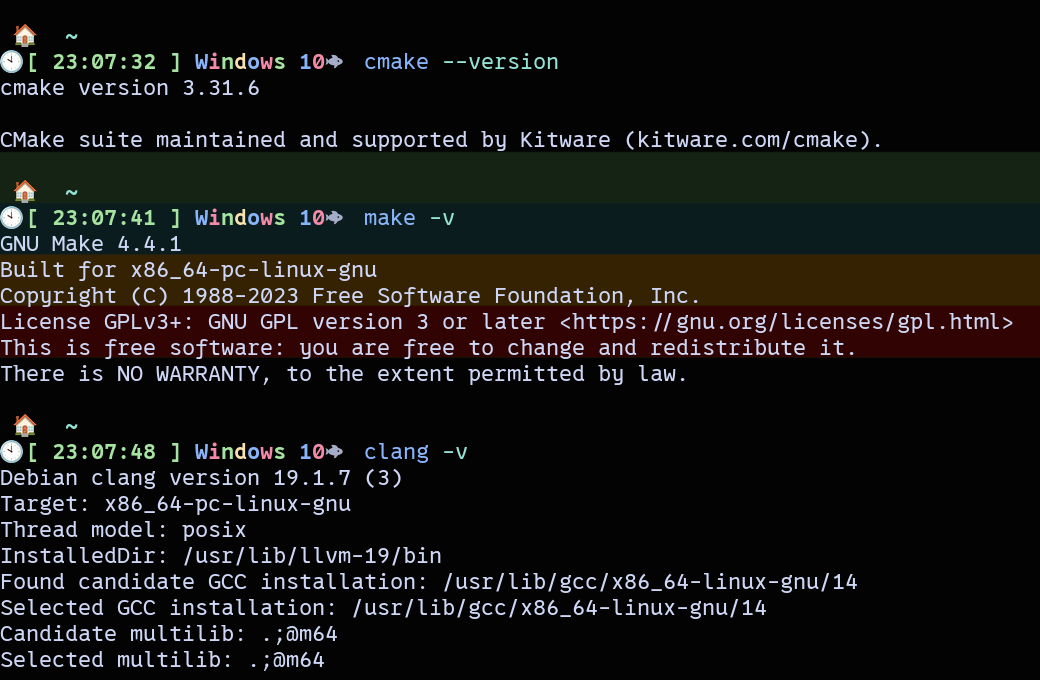
\includegraphics[width=0.95\textwidth]{images/chapters/dependencies.png}
		      \caption{安装基础依赖}
		      \label{fig:dependencies}
	      \end{figure}
\end{enumerate}

\subsection{代码实现}
\begin{itemize}
	\item 定义变量类型
	      \begin{itemize}
		      \item \begin{lstlisting}
            point = Tuple[int, int]
            capsule = Tuple[point, point, int]
            \end{lstlisting}
		      \item 选择一个素数的循环群，是群的生成元。
		            该软件系统选择我国商用密码选定的素数域椭圆曲线的参数，如图\ref{fig:sm2_parameter}所示：
		            \begin{figure}[H]
			            \begin{center}
				            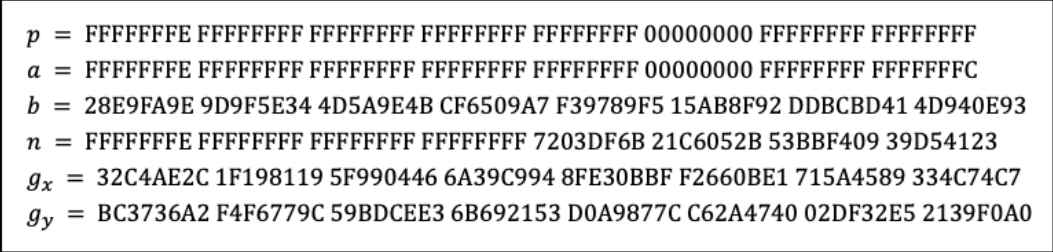
\includegraphics[width=0.95\textwidth]{images/chapters/sm2_parameter.png}
			            \end{center}
			            \caption{国密SM2椭圆曲线参数}\label{fig:sm2_parameter}
		            \end{figure}
	      \end{itemize}
	\item 定义椭圆曲线上的运算
	      \begin{lstlisting}
          multiply(a: point, n: int) -> point: # 椭圆曲线上的倍点运算

          add(a: point, b: point) -> point: # 椭圆曲线上，两个点的加法运算

          inv(a: int, n: int) -> int: # 椭圆曲线上，求a关于素数p的逆元运算

          Z_q = (0, sm2p256v1.N - 1)

          g = (sm2p256v1.Gx, sm2p256v1.Gy)

          U = multiply(g, random.randint(0, sm2p256v1.N - 1))
          \end{lstlisting}

	\item 哈希函数
	      \begin{lstlisting}
          hash2(double_G: Tuple[point, point]) -> int: G^2 -> Z_q

          hash3(triple_G: Tuple[point, point, point]) -> int: G^3 -> Z_q

          hash4(triple_G: Tuple[point, point, point], Z_q:int) -> int: G^3*Z_q -> Z_q

          hash5(id:int, D:int) -> int:

          hash6(triple_G: Tuple[point, point, point]) -> int:
        \end{lstlisting}
\end{itemize}

\subsection{python库调用与类型定义}
GmSSL是由我国自主开发的国产商用密码开源库，实现了对国密算法、标准和安全通信协议的全面功能覆盖，
支持包括移动端在内的主流操作系统和处理器，支持密码钥匙、密码卡等典型国产密码硬件，
提供功能丰富的命令行工具及多种编译语言编程接口。本算法中使用了其中的SM2,SM3,SM4函数。
如图\ref{fig:gmssl}所示：
\begin{figure}[H]
	\begin{center}
		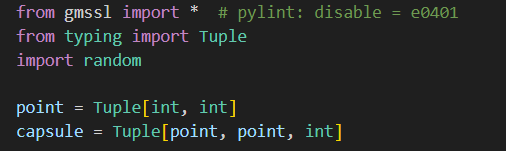
\includegraphics[width=0.95\textwidth]{images/chapters/gmssl.png}
	\end{center}
	\caption{库引用与类型定义}\label{fig:gmssl}
\end{figure}

定义国密标准的SM2类参数和曲线上的生成元$g$, $U$。
如图\ref{fig:sm2_python_parameter}所示。
\begin{figure}[H]
	\begin{center}
		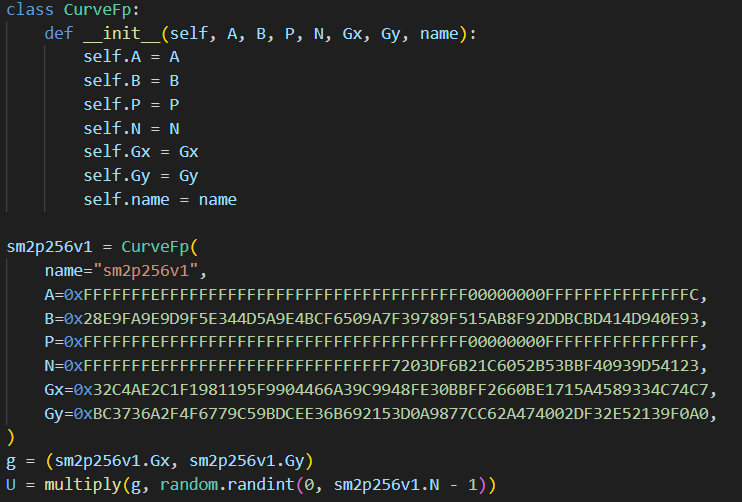
\includegraphics[width=0.95\textwidth]{images/chapters/sm2_python_parameter.png}
	\end{center}
	\caption{国密标准的SM2类参数}\label{fig:sm2_python_parameter}
\end{figure}


\subsection{国密算法椭圆曲线上的加法、倍乘、求逆元}
通过利用雅各比坐标系，将椭圆曲线上的点从仿射坐标转换为射影坐标表示，
减少了点运算中的模逆运算次数，从而显著提高了椭圆曲线上点的计算效率。
如图\ref{fig:sm2_methods}所示：
\begin{figure}[H]
	\begin{center}
		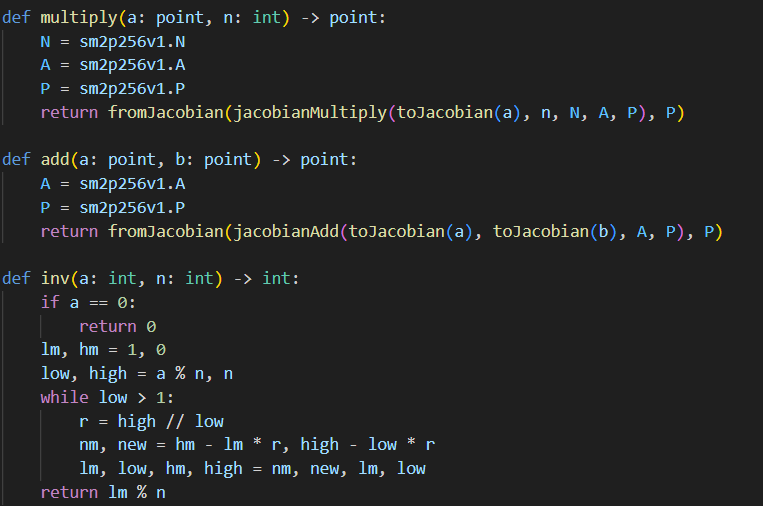
\includegraphics[width=0.95\textwidth]{images/chapters/sm2_methods.png}
	\end{center}
	\caption{SM2椭圆曲线的加法、倍乘、求逆}\label{fig:sm2_methods}
\end{figure}

\subsection{hash函数}
hash2(),hash3(),hash4()函数分别接受包含两个椭圆曲线点的元组、
三个椭圆曲线点的元组、三个椭圆曲线点的元组和一个整数$Z_q$作为输入。
然后使用SM3哈希函数初始化。遍历$double_G$中的每个点并对其坐标进行哈希处理，
hash4()需要再对整数$Z_q$进行哈希处理。最后返回处理后的整数哈希值。
如图\ref{fig:hashes}所示：
\begin{figure}[H]
	\begin{center}
		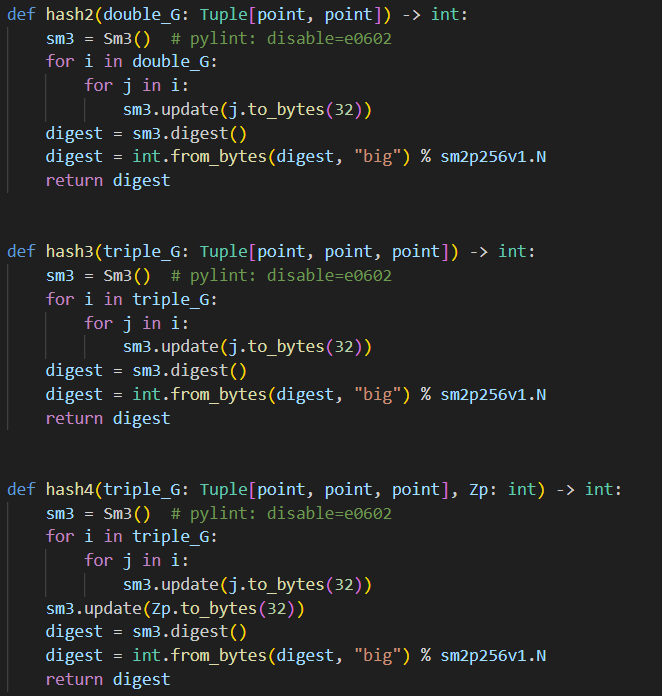
\includegraphics[width=0.95\textwidth]{images/chapters/hashes.png}
	\end{center}
	\caption{hash2(),hash3(),hash4函数}\label{fig:hashes}
\end{figure}

\subsection{密钥派生函数}
KDF()函数首先接受一个椭圆曲线点$G$作为输入。然后使用SM3哈希函数进行初始化，
遍历$G$的坐标并对其进行哈希处理。将哈希输出转换为大整数并模$sm2p256v1.N$取值。
最后使用一个128位的掩码来获取哈希输出的前128位，返回处理后的整数哈希值。
如图\ref{fig:kdf}所示：
\begin{figure}[H]
	\begin{center}
		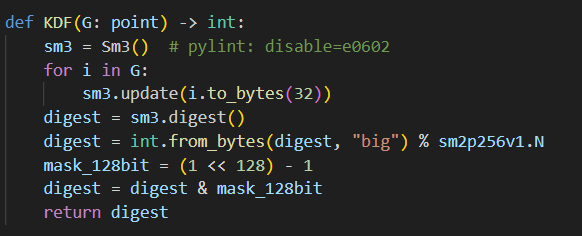
\includegraphics[width=0.95\textwidth]{images/chapters/kdf.png}
	\end{center}
	\caption{KDF()函数}\label{fig:kdf}
\end{figure}

\subsection{密钥封装函数}
首先生成随机整数$r,u$，在椭圆曲线上计算$E,V$。然后计算$s=(u + r \cdot \text{hash2}((E, V))) \bmod \text{sm2p256v1.N}$。
计算共享秘密$\text{pk}_A \cdot (r + u)$，然后使用KDF函数从该共享秘密派生出共享密钥$K$。
构造封装体$\text{capsule}$，封装体由$(E,V,s)$组成。最后函数返回一个元组，其中包含派生的共享密钥和封装体。
如图\ref{fig:encapsulate}所示：
\begin{figure}[H]
	\begin{center}
		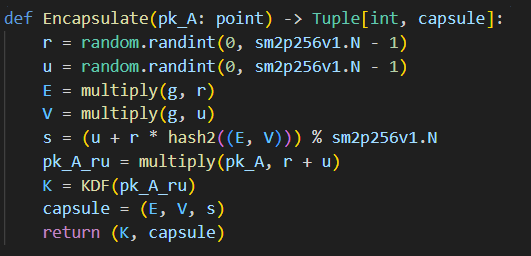
\includegraphics[width=0.95\textwidth]{images/chapters/encapsulate.png}
	\end{center}
	\caption{密钥封装函数}\label{fig:encapsulate}
\end{figure}

\subsection{密钥对生成函数}
首先初始化SM2密钥对生成器，调用generate\_key()方法来生成密钥对。
从生成的公钥中提取$x$和$y$坐标，并将它们从字节转换为整数；提取生成的私钥，
并将其从字节转换为整数。最后返回一个元组，其中包含公钥（作为坐标对）和私钥（作为整数）。
如图\ref{fig:generate_key_pair}所示：
\begin{figure}
	\begin{center}
		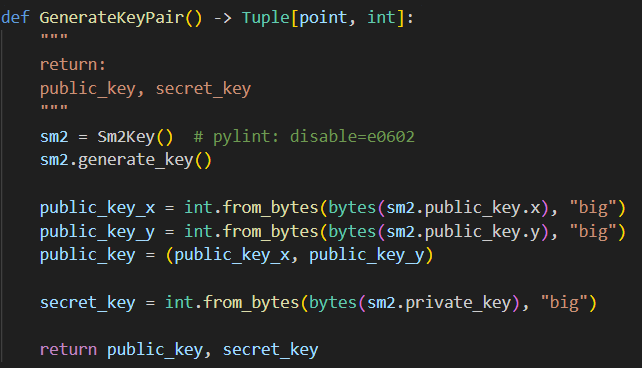
\includegraphics[width=0.95\textwidth]{images/chapters/generate_key_pair.png}
	\end{center}
	\caption{密钥对生成函数}\label{fig:generate_key_pair}
\end{figure}

\subsection{加密函数}
首先，函数通过Encapsulate(pk)方法进行封装，将公钥与随机性结合，产生一个共享的秘密$K$和一个公开的封装体capsule。
然后验证密钥长度，确保从封装体中得到的秘密密钥$K$的长度确实为 16 字节。如果不是，将抛出一个错误。
设置一个固定的初始化向量iv，然后使用SM4对称加密算法（在CBC模式下）与密钥$K$和iv进行初始化。
这里，DO\_ENCRYPT是一个指示加密操作的常量。使用初始化后的SM4加密实例对消息$m$进行加密。
最后函数返回一个元组，其中包含公开的封装体和加密后的数据。

加密函数使用了混合加密方案：首先使用非对称加密（封装）产生一个共享的秘密，然后使用该秘密进行对称加密。
这种方式结合了非对称加密的安全性和对称加密的效率。
如图\ref{fig:enc}所示：
\begin{figure}[H]
	\begin{center}
		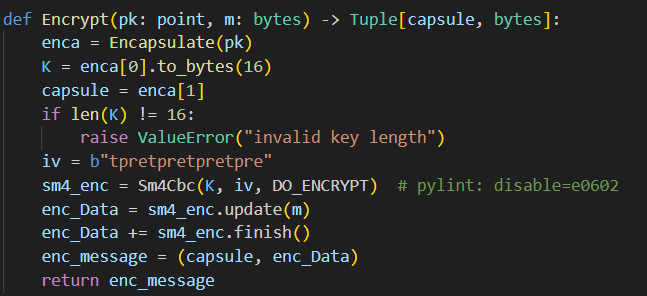
\includegraphics[width=0.95\textwidth]{images/chapters/enc.png}
	\end{center}
	\caption{加密函数}\label{fig:enc}
\end{figure}

\subsection{解封装函数}
该函数的目的是使用私钥$\text{sk}_A$解封提供的封装体$\text{capsule}$，以恢复原始的共享密钥。
首先从封装体$\text{capsule}$中提取$E,V,s$。然后在椭圆曲线上计算$(E+V)^{\text{sk}_A}$，
最后使用KDF函数对其解密，得到共享密钥$K$。
如图\ref{fig:decapsulate}所示：
\begin{figure}[H]
	\begin{center}
		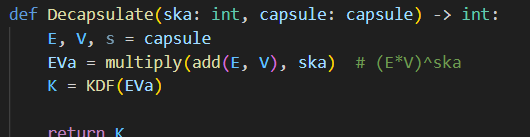
\includegraphics[width=0.95\textwidth]{images/chapters/decapsulate.png}
	\end{center}
	\caption{解封装函数}\label{fig:decapsulate}
\end{figure}

\subsection{解密函数}
该函数的目的是使用私钥$\text{sk}_A$解密密文$C$。
首先从加密数据$C$中提取封装体$\text{capsule}$和加密的数据$\text{enc\_Data}$。
然后使用$\text{Decapsulate}$函数和私钥$\text{sk}_A$解封$\text{capsule}$以恢复共享的秘密密钥$K$。
使用恢复的密钥$K$和固定的初始化向量$\text{iv}$，然后初始化$\text{SM4}$对称解密算法（在$\text{CBC}$模式下）。
使用初始化后的$\text{SM4}$解密实例解密$\text{enc\_Data}$，函数返回解密后的数据$\text{dec\_Data}$。

解密函数先解封了一个封装体以恢复对称密钥$K$，然后使用这个密钥解密提供的加密数据。
这是混合加密方案的一个典型应用，结合了非对称加密的安全性和对称加密的效率。
如图\ref{fig:dec}所示：
\begin{figure}[H]
	\begin{center}
		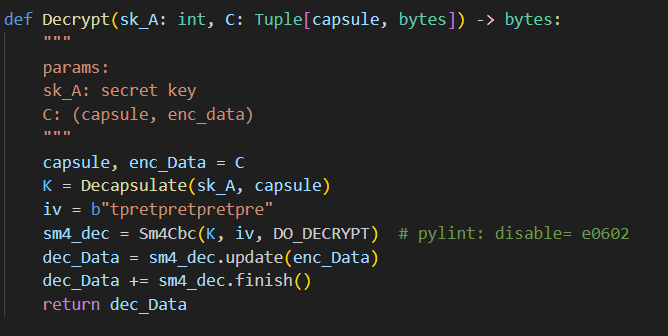
\includegraphics[width=0.95\textwidth]{images/chapters/dec.png}
	\end{center}
	\caption{解密函数}\label{fig:dec}
\end{figure}

\subsection{hash5()函数}
该函数的目的是利用两个整数$\text{id}$和$D$生成一个哈希值。首先初始化 SM3 哈希算法实例。
然后将整数$\text{id}$转换为 32 字节的字节串，并更新哈希算法；将整数$D$转换为 32 字节的字节串，
并更新哈希算法。完成哈希计算并获取结果作为字节串。将字节串的哈希结果转换为整数，
并进行模运算以确保结果在$\text{sm2p256v1.N}$范围内。函数返回计算得到的哈希值。
如图\ref{fig:hash5}所示：
\begin{figure}[H]
	\begin{center}
		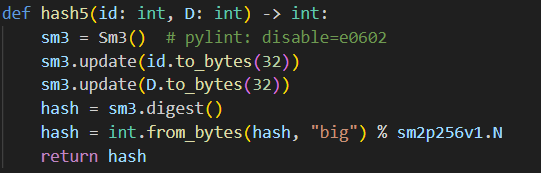
\includegraphics[width=0.95\textwidth]{images/chapters/hash5.png}
	\end{center}
	\caption{hash5()函数}\label{fig:hash5}
\end{figure}

\subsection{hash6()函数}
该函数的目的是从一个包含三个点的元组$\text{triple\_G}$生成一个哈希值。首先初始化 SM3 哈希算法实例。
然后对于$\text{triple\_G}$中的每个点$i$，再对该点中的每个坐标执行以下操作：将坐标转换为 32 字节的字节串，
并更新哈希算法。完成哈希计算并获取结果作为字节串。将字节串的哈希结果转换为整数，
并进行模运算以确保结果在$sm2p256v1.N$范围内。最后函数返回计算得到的哈希值。
如图\ref{fig:hash6}所示：
\begin{figure}[H]
	\begin{center}
		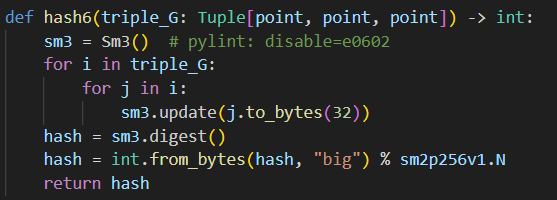
\includegraphics[width=0.95\textwidth]{images/chapters/hash6.png}
	\end{center}
	\caption{hash6()函数}\label{fig:hash6}
\end{figure}

\subsection{多项式函数}
该函数计算了一个关于的多项式的值，其中多项式的系数在$f\_modulus$列表中。
然后，它对结果进行了模$sm2p256v1.N$运算。
如图\ref{fig:polynomial}所示：
\begin{figure}
	\begin{center}
		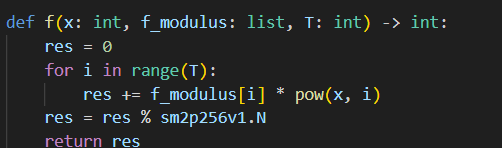
\includegraphics[width=0.95\textwidth]{images/chapters/polynomial.png}
	\end{center}
	\caption{多项式生成函数}\label{fig:polynomial}
\end{figure}

\subsection{重加密密钥生成函数}
随机生成一个整数$x_A$作为临时私钥。使用这个临时私钥计算其对应的公钥$X_A$。
通过哈希函数$\text{hash3()}$得到$d$然后使用公钥、私钥和$d$来计算$r_0$，
它是多项式的第一个系数。其余的系数随机生成。
而$D$是Alice和Bob的公钥之间的另一个Diffie-Hellman密钥交换的结果。

计算KF这部分的逻辑循环对$N$次循环，每次都会为KF列表生成一个新条目。
每次迭代都会随机生成一个值$y$，并计算与之相关的公钥$Y$。通过hash5计算$s\_x$得出哈希值。
然后计算$U_1$。将所有这些值打包为一个元组kFrag，并添加到KF列表中。
如图\ref{fig:generate_rekey}所示：
\begin{figure}[H]
	\begin{center}
		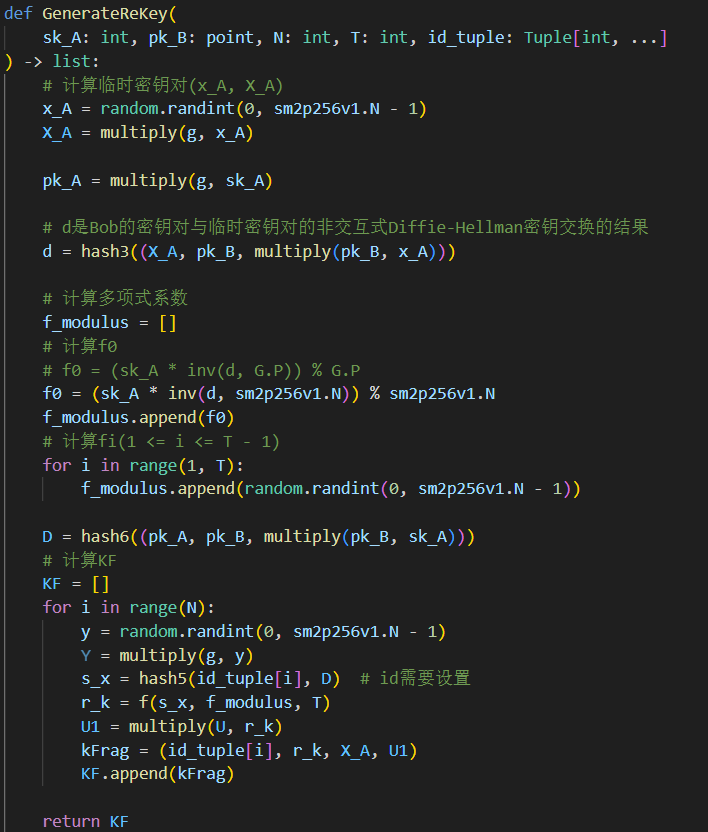
\includegraphics[width=0.95\textwidth]{images/chapters/generate_rekey.png}
	\end{center}
	\caption{重加密密钥生成函数}\label{fig:generate_rekey}
\end{figure}

\subsection{capsule检查函数}
该函数的目的是验证所提供的capsule是否有效。在密钥封装机制(KEM)中，
验证胶囊的有效性是关键的一步，以确保密钥的正确性和完整性。

首先解包胶囊，通过结构化赋值，将胶囊元组的三个组成部分提取为变量$E$,$V$,$s$。
然后使用哈希函数hash2()计算$E$和$V$的哈希值，结果存储在$h2$中。
验证等式$g^s=V\cdot E^{\text{hash2}(E,V)}$是否成立。如果成立，则将flag设置为True，否则设置为False。
最后函数返回一个布尔值flag来表示胶囊是否有效。
如图\ref{fig:check_capsule}所示：
\begin{figure}[H]
	\begin{center}
		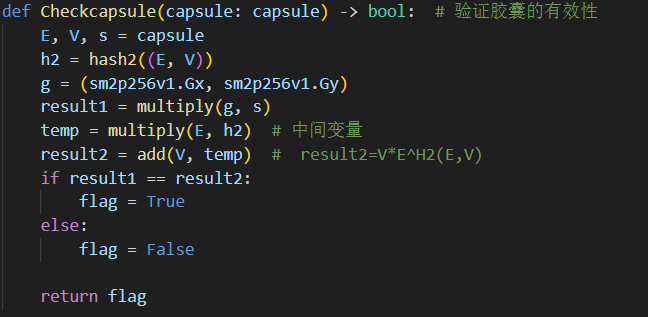
\includegraphics[width=0.95\textwidth]{images/chapters/check_capsule.png}
	\end{center}
	\caption{检查函数}\label{fig:check_capsule}
\end{figure}

\subsection{重封装算法}
首先输入参数kFrag和capsule，提取元组的内容:从kFrag中提取出id，rk，
$X_A$，$U_1$；从capsule中提取出$E$，$V$，$s$。然后使用Checkcapsule()函数验证提供的胶囊的有效性。
如果胶囊无效，函数会抛出一个错误。否则计算$E_1$和$V_1$。
最后使用$E_1$，$V_1$，id，$X_A$创建一个新的元组cfrag，并作为返回值。
如图\ref{fig:reencapsulate}所示：
\begin{figure}
	\begin{center}
		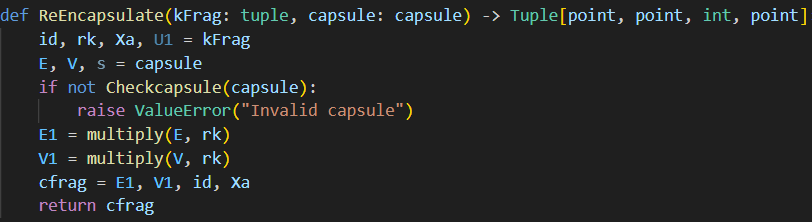
\includegraphics[width=0.95\textwidth]{images/chapters/reencapsulate.png}
	\end{center}
	\caption{重封装算法}\label{fig:reencapsulate}
\end{figure}

\subsection{重加密函数}
ReEncrypt()是重加密函数，接受一个密钥片段kFrag和一个由胶囊与加密数据组成的密文元组作为输入。
在函数内部，首先从C提取出胶囊和加密数据。然后，使用ReEncapsulate()函数处理kFrag和胶囊，生成cFrag。
最后，该函数返回一个包含cFrag和原始加密数据的重加密密文元组。
如图\ref{fig:reenc}所示：
\begin{figure}[H]
	\begin{center}
		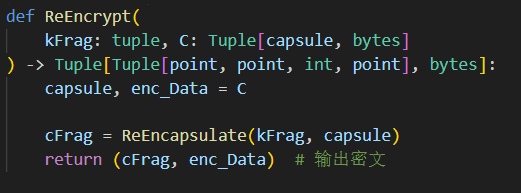
\includegraphics[width=0.95\textwidth]{images/chapters/reenc.png}
	\end{center}
	\caption{重加密函数}\label{fig:reenc}
\end{figure}

\subsection{重加密密文聚合函数}
该函数的功能是将一个由cFrag和ct (enc\_Data)
组成的重加密密文片段元组列表转化为一个包含两个元素的列表：
第一个元素是所有cFrag的列表，第二个元素是第一个元组的ct值。
如图\ref{fig:mergecfrag}所示：
\begin{figure}[H]
	\begin{center}
		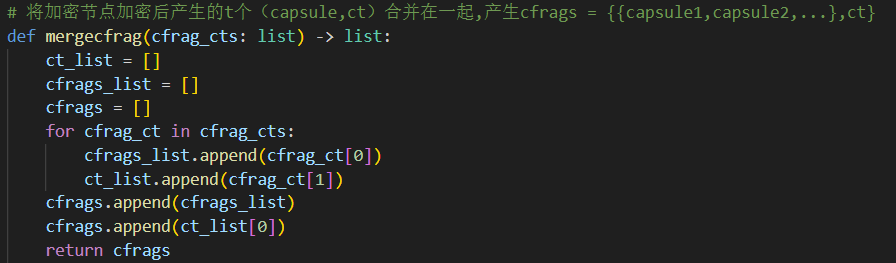
\includegraphics[width=0.95\textwidth]{images/chapters/mergecfrag.png}
	\end{center}
	\caption{重加密密文聚合函数}\label{fig:mergecfrag}
\end{figure}

\subsection{重封装解封函数}
DecapsulateFrag()是一个重封装解封函数，它接受B的私钥sk$_B$，B和A的公钥pk$_B$，pk$_A$，
以及一个包含密文片段的列表cFrags作为输入参数。在函数内部，
首先从cFrags中提取出各自的信息并存放到四个列表Elist，Vlist，idlist，$X_A$list中。
然后，函数计算pk$_A$与sk$_B$在椭圆曲线上的乘积，并基于此生成$D$值。
接下来，它生成一个名为s$_X$的列表，其中每个元素都是基于idlist列表的每个id得到的。
然后函数进一步计算多个系数b并存储在bis列表中。使用这些系数，计算出$E_2$，$V_2$的值。
后续，在椭圆曲线上进行更多的点乘操作以计算$X'_a$和$d$值。
最后，函数在椭圆曲线上将$E_2$，$V_2$相加并乘$d$值，
然后使用KDF函数从结果中派生出密钥$K$，并返回该密钥。
如图\ref{fig:decapsulatefrag}所示：
\begin{figure}
	\begin{center}
		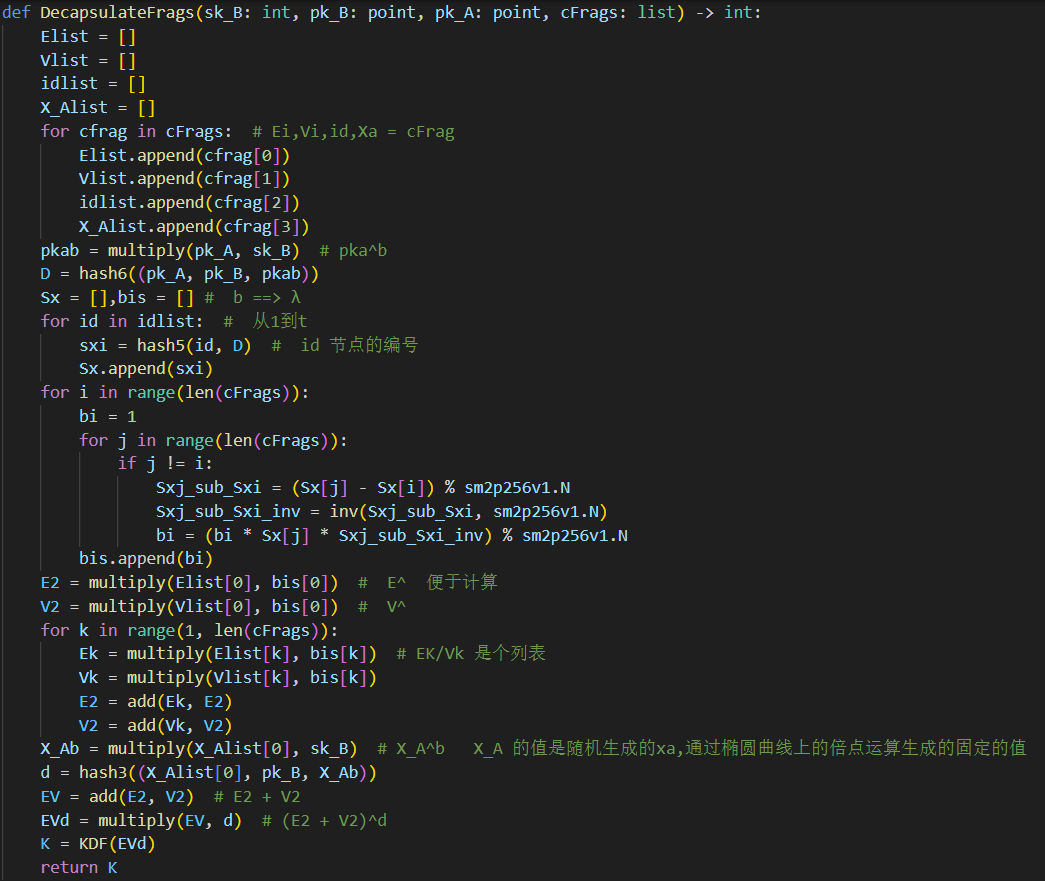
\includegraphics[width=0.95\textwidth]{images/chapters/decapsulatefrags.png}
	\end{center}
	\caption{重封装解封函数}\label{fig:decapsulatefrag}
\end{figure}

\subsection{重加密解密函数}
DecryptFrags()是重加密解密函数，它使用B的私钥sk$_B$、B和A的公钥pk$_B$，
pk$_A$以及一个包含密文片段的列表cfrags作为输入。在函数内部，首先从cfrags中提取密文片段，
得到capsules和enc$_{Data}$。然后使用DecapsulateFrags()函数从capsules中解封装出密钥K。
然后，将此密钥转换为16字节的字节串。最后使用SM4的CBC模式以及提取出的密钥来初始化解密算法，
并解密enc$_{Data}$生成重加密解密数据dec$_{Data}$。如果在解密过程中遇到错误，
函数会捕获并打印错误消息，并设置解密数据dec$_{Data}$为一个空字节串。
最后，返回解密后的数据dec$_{Data}$。
如图\ref{fig:decryptfrags}所示：
\begin{figure}[H]
	\begin{center}
		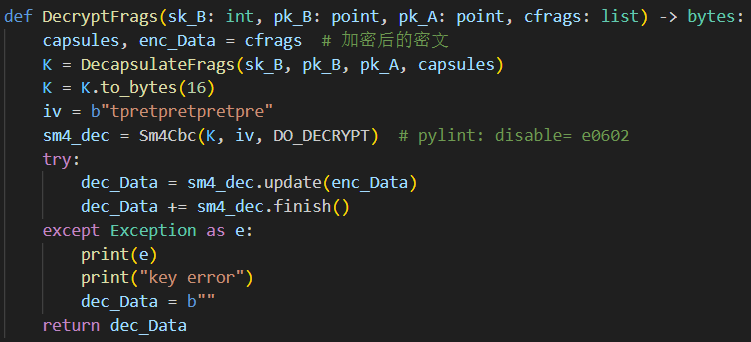
\includegraphics[width=0.95\textwidth]{images/chapters/decfrags.png}
	\end{center}
	\caption{重加密解密函数}\label{fig:decryptfrags}
\end{figure}

\subsection{系统流程}

\begin{enumerate}
	\item 数据拥有方生成公私钥对并加密数据
	\item 数据请求方向拥有方申请访问权限
	\item 拥有方同意后生成重加密密钥片段
	\item 代理节点执行重加密操作
	\item 数据请求方接收并解密数据
\end{enumerate}
系统流程图如图\ref{fig:system_flow}所示：
\begin{figure}[H]
	\begin{center}
		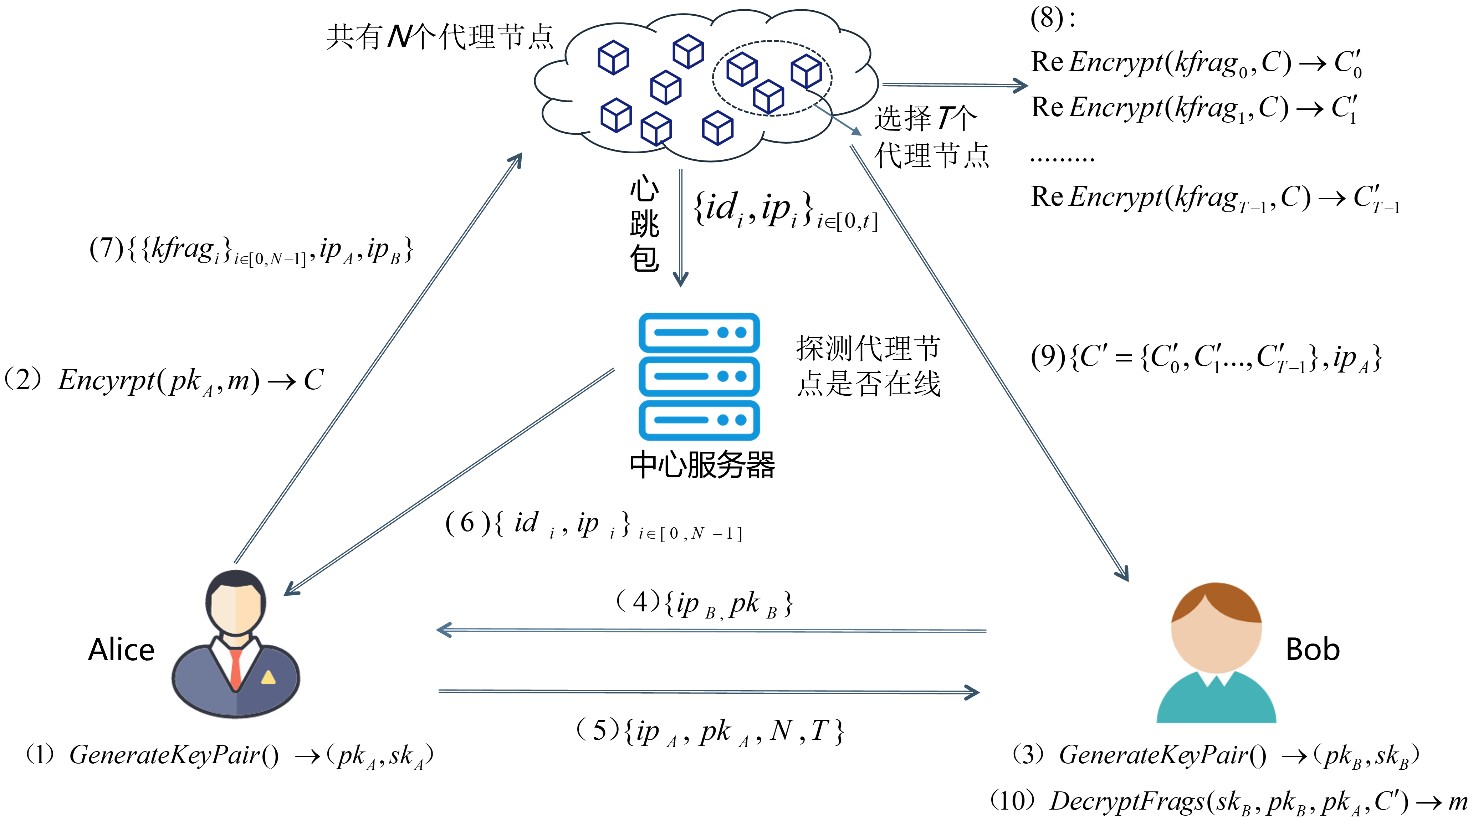
\includegraphics[width=0.95\textwidth]{images/chapters/system_flow.png}
	\end{center}
	\caption{系统流程图}
	\label{fig:system_flow}
\end{figure}


\subsection{关键模块}
本系统的功能实现依赖于多个专用模块的协同工作，每个模块负责特定的功能领域，
通过标准化接口相互配合，共同构建完整的代理重加密框架。
这种模块化设计不仅提高了系统的可维护性和可扩展性，还便于针对不同应用场景进行定制化部署。

\subsubsection{密钥管理模块}
密钥管理模块作为系统安全基础设施的核心组件，负责整个系统的密码材料全生命周期管理。
该模块首先实现了基于SM2算法的公私钥对生成功能，支持用户身份绑定的密钥派生和随机密钥生成两种方式。
在密钥生成过程中，模块采用符合密码学要求的高质量随机源，确保生成密钥的不可预测性和唯一性。
对于高安全需求场景，系统支持与硬件安全模块(HSM)或可信平台模块(TPM)集成，
将密钥生成过程迁移至物理隔离的安全环境中执行，进一步增强密钥材料的安全性。

该模块还承担重加密密钥的管理职责，包括基于用户授权关系动态生成重加密密钥、
执行基于Shamir秘密共享的密钥分片、协调密钥片段的安全分发以及处理密钥的定期更新与撤销。
特别是在密钥更新机制中，系统实现了无缝的版本转换策略，确保密钥更新不影响已加密数据的可访问性，
同时支持紧急情况下的密钥撤销，有效限制安全事件的影响范围。

在密钥存储方面，模块采用多层次的安全防护措施。所有敏感密钥材料在存储前均经过额外加密处理，
加密密钥通过密钥派生函数从用户主密钥和随机盐值派生，并使用安全的密钥封装机制保护。
系统对存储介质进行了安全分级，核心私钥仅保存在高安全级别的受控环境中，
而公钥和非敏感元数据可分布在普通存储系统中。模块还实现了完整的密钥备份与恢复机制，
在确保业务连续性的同时，通过严格的访问控制和审计日志记录，防止备份成为安全漏洞。

\subsubsection{加解密模块}
加解密模块提供了系统的核心密码学功能，通过标准化的接口封装各种密码算法，
为上层应用提供统一的加密服务。该模块首先实现了对国密算法族（SM2/SM3/SM4）的全面封装，
提供了符合国家标准规范的算法实现。在接口设计上，模块采用了易于使用的面向对象模式，
隐藏了底层密码学操作的复杂性，同时保留了必要的参数配置灵活性，
满足不同安全级别和性能需求的应用场景。

该模块的核心功能是实现高效的混合加密机制，将SM2和SM4算法有机结合，
在保证安全性的前提下优化性能表现。具体而言，对于需要加密的原始数据，
系统首先随机生成一个高熵值的SM4会话密钥，使用该密钥和GCM模式对数据进行对称加密；
然后使用接收方的SM2公钥对会话密钥本身进行非对称加密。
这种设计使得系统能够高效处理大规模数据，同时保持密钥管理的灵活性。在实现上，
模块采用流水线处理和内存映射技术处理大文件，提供了分块加密和并行处理能力，
显著提升了系统在大数据环境下的性能。

加解密模块还提供了一系列辅助功能，包括数据完整性验证、安全随机数生成、
密码学签名与验证等，构成了完整的密码服务体系。特别是在数据完整性保护方面，
模块利用SM3算法和HMAC机制实现了强认证，确保数据在传输和存储过程中不被篡改。
模块的接口设计考虑了与各类应用场景的兼容性，提供了同步/异步调用模式、
批处理接口和流式处理能力，满足从嵌入式设备到大型服务器的多种部署环境需求。

\subsubsection{代理重加密模块}
代理重加密模块是系统实现安全数据共享的核心组件，负责执行密文转换操作而无需解密原始数据。
该模块基于门限代理重加密理论，实现了$(t,n)$门限重加密方案，
要求至少$t$个代理节点协作才能完成重加密过程。
模块的设计确保单个代理节点无法获取足够信息来解密数据或重构完整的重加密密钥，
从而有效防止了代理节点的权限滥用。

在重加密密钥管理方面，模块实现了密钥片段的安全存储和访问控制机制。
每个代理节点仅存储分配给它的重加密密钥片段，
这些片段通过额外的加密层和节点本地的安全存储机制保护。模块支持密钥片段的定期更新和版本控制，
实现了前向安全性，即使某个时间点的密钥片段被泄露，也不会危及后续操作的安全性。

代理重加密模块的另一重要功能是协调多节点共同完成重加密操作。
当系统接收到重加密请求时，模块首先验证请求的合法性和授权状态，然后启动分布式重加密协议。
在该协议中，参与节点各自使用本地存储的密钥片段对密文进行部分重加密，并生成重加密证明；
协调节点收集这些部分结果，在达到门限数量后，组合生成最终的重加密结果。
整个过程采用安全多方计算技术确保中间结果不泄露敏感信息，
同时通过零知识证明验证各节点的操作正确性，防止恶意节点提交错误结果。

模块还实现了丰富的异常处理和容错机制，能够应对节点失效、网络中断等各类故障场景，
确保系统在不理想的网络环境中仍能可靠运行。性能优化方面，模块采用了批处理重加密、
预计算和结果缓存等技术，有效降低了重加密操作的延迟和资源消耗。

\subsubsection{通信模块}
通信模块为系统各组件提供了统一的数据交换基础设施，负责处理节点间的消息传递和状态同步。
该模块基于HTTP/HTTPS协议构建，充分利用了Web技术的成熟性和广泛兼容性，
便于跨平台部署和防火墙穿透。在具体实现上，模块采用RESTful API设计风格，
定义了清晰的资源模型和操作语义，支持标准的HTTP方法（GET、POST、PUT、DELETE等）进行资源操作。

安全通信是该模块的核心关注点，系统实现了多层次的安全防护机制。在传输层，
所有通信均采用TLS 1.3协议加密，确保数据传输的机密性和完整性；在应用层，
模块实现了基于JWT（JSON Web Token）的身份认证和访问控制，
每个请求都需要携带有效的身份令牌和操作授权证明。为防止重放攻击和中间人攻击，
系统还采用了请求时间戳验证、请求签名和随机挑战响应机制。针对分布式拒绝服务攻击，
模块实现了请求频率限制和资源隔离策略，有效保护系统的可用性。

模块支持灵活的异步数据传输模式，特别适合处理长时间运行的重加密操作和大文件传输场景。
在异步模式下，系统返回操作标识符，客户端可以通过该标识符查询操作状态或接收操作完成通知，
避免了长连接占用和请求超时问题。为提高通信效率，模块实现了消息压缩、
批量请求处理和连接池管理等优化技术，显著降低了网络带宽消耗和请求处理延迟。

在可靠性方面，通信模块采用了完整的错误处理和重试机制，能够应对网络波动和临时故障。
系统定义了统一的错误码和响应格式，提供了详细的错误信息和处理建议，便于问题诊断和自动恢复。
模块还实现了通信事件的详细日志记录和性能指标收集，为系统监控和性能优化提供了数据支持。

\section{安全性分析}
系统安全性是代理重加密解决方案的核心考量，通过多层次、纵深防御的安全架构，
系统在保障数据共享效率的同时，确保了信息资产的全面保护。
安全性分析从多个维度评估了系统的风险抵抗能力和安全保障水平。

系统的底层安全基础建立在国密算法的密码学强度上。SM2椭圆曲线密码算法采用256位密钥长度，
其安全性基于椭圆曲线离散对数问题，当前最优算法的计算复杂度为$O(2^{128})$，
远超现有技术能力。SM3哈希算法输出256位杂凑值，提供了强抗碰撞性和抗前像性，
有效保障了数据完整性验证机制的安全性。SM4分组密码通过32轮非线性迭代提供了高强度的数据保密性，
经过密码学分析验证能够抵抗已知的各类密码攻击。这些国家标准算法经过严格的安全评估和论证，
既符合国内密码合规要求，又提供了国际认可的安全强度，为系统奠定了坚实的密码学基础。

分布式架构是系统抵抗单点故障和集中式攻击的关键机制。与传统中心化系统不同，
本方案将关键功能和敏感数据分散到多个独立节点，
任何单点的妥协都不会导致整个系统的崩溃或安全机制的完全失效。特别是在代理重加密过程中，
重加密密钥和操作被分散到多个代理节点，攻击者需要同时控制多个节点才能获取有效信息，
显著提高了攻击难度。系统通过一致性协议和状态同步机制，确保分布式环境下的操作一致性和数据完整性，
即使部分节点失效或遭受攻击，系统仍能维持安全运行。
分布式架构还提供了自然的负载均衡和横向扩展能力，有效防止了资源耗尽型攻击，
提高了系统整体的可用性和鲁棒性。

门限机制为系统提供了细粒度的容错能力和访问控制。通过$(t,n)$门限方案，
系统可以在保证安全性的前提下，容忍最多$n-t$个节点的失效或恶意行为。
这种设计既增强了系统的可用性，又提高了安全边界，形成了"多数决策"的信任模型。
在实际部署中，门限参数可以根据具体应用场景的安全需求和可用性要求进行灵活配置，
实现安全性和可用性的最优平衡。门限机制还支持动态成员管理，
允许在系统运行过程中添加或移除参与节点，而不需要重建整个密钥体系，
提供了良好的运维灵活性。

完整性校验是防止数据篡改和确保系统可信运行的重要保障。系统在多个层次实现了数据完整性验证：
从基础的SM3哈希验证，到高级的数字签名和认证加密。
所有关键数据在传输和存储过程中均附带密码学完整性证明，
任何未授权的修改都会导致验证失败并触发安全警报。特别是在代理重加密过程中，
系统实现了操作证明机制，每个参与节点都需要提供其操作正确性的零知识证明，
这些证明可以被其他节点或审计者验证，确保了整个重加密过程的可验证性和不可抵赖性。
系统还建立了完整的审计日志链，记录所有关键操作和状态变更，支持事后追溯和责任认定。

通过这些多层次、相互补充的安全机制，系统构建了全面的安全防护体系，在算法层面、
架构层面和应用层面均提供了充分的安全保障，有效应对各类安全威胁和攻击场景。

\section{本章小结}
本章详细介绍了系统的设计方案和实现细节，包括总体架构、核心算法、关键技术和具体实现。
通过合理的系统设计和可靠的技术实现，
确保了系统在分布式环境下能够安全高效地完成数据共享和授权管理任务

\chapter{系统测试与结果分析}

\section{测试环境}

\subsection{本地测试环境}

本系统在以下环境中进行本地测试：

\begin{table}[h]
	% FIX:需要更新windows测试环境
	\centering
	\caption{本地系统环境}
	\begin{tabular}{ll}
		\hline
		\textbf{计算机系统} & \textbf{版本}                               \\
		\hline
		处理器            & Intel(R) Core(TM) i7-10750H CPU @ 2.60GHz \\
		操作系统           & Windows 10                                \\
		\hline
		\textbf{软件}    & \textbf{版本}                               \\
		\hline
		Python         & 3.8.0                                     \\
		gmssl          & 3.2.1                                     \\
		SQLite         & 3.39.3                                    \\
		\hline
	\end{tabular}
\end{table}

\begin{table}[h]
	\centering
	\caption{本地系统环境2}
	\begin{tabular}{ll}
		\hline
		\textbf{计算机系统} & \textbf{版本}                      \\
		\hline
		处理器            & AMD Ryzen 5 4500U (6) @ 2.38 GHz \\
		操作系统           & Kali GNU/Linux Rolling x86\_64   \\
		\hline
		\textbf{软件}    & \textbf{版本}                      \\
		\hline
		Python         & 3.13.3                           \\
		gmssl          & 3.2.1                            \\
		SQLite         & 3.39.3                           \\
		\hline
	\end{tabular}
\end{table}

\subsection{云端测试环境}

云端测试采用华为云服务器，具体配置如下：

\begin{table}[h]
	\centering
	\caption{云端系统环境}
	\begin{tabular}{ll}
		\hline
		\textbf{服务器} & \textbf{配置}   \\
		\hline
		规格           & 2vCPUs | 4GiB \\
		\hline
		\textbf{软件}  & \textbf{版本}   \\
		\hline
		Docker       & 24.0.5        \\
		Redis        & 7.0.11        \\
		Node.js      & 18.16.0       \\
		\hline
	\end{tabular}
\end{table}

\section{功能测试}
\subsection{密钥生成与管理测试}
测试了系统的密钥生成和管理功能，包括：
\begin{enumerate}
	\item 公私钥对生成
	\item 重加密密钥生成
	\item 密钥分发和存储
\end{enumerate}
测试结果表明，系统能够正确生成和管理各类密钥，确保密钥的唯一性和安全性。

\subsection{加密解密测试}
对系统的加密解密功能进行了全面测试：
\begin{enumerate}
	\item 原始数据加密
	\item 重加密操作
	\item 密文合并
	\item 解密验证
\end{enumerate}
测试结果显示，系统能够正确完成各类加解密操作，保证数据的机密性和完整性。

\section{性能测试}

\subsection{算法性能测试}

在不同节点数(N)和门限值(T)配置下进行测试，主要测试指标包括：
\begin{enumerate}
	\item 算法总运行时间
	\item 密钥生成时间
	\item 加密算法时间
	\item 重加密密钥生成时间
	\item 重加密算法时间
	\item 解密算法时间
\end{enumerate}

测试结果显示：
\begin{enumerate}
	% FIX: 需要进行大规模测试
	\item 当N=20，T=10时，系统性能最优
	\item 算法执行时间远小于1秒的性能要求
	\item 随着节点数增加，系统仍保持良好的扩展性
\end{enumerate}

\subsection{系统响应时间测试}
对系统在云端环境下的响应性能进行测试：
\begin{enumerate}
	\item 异步处理数据时间
	\item 通信延迟
	\item 并发处理能力
\end{enumerate}
测试结果表明系统具有良好的响应性能和并发处理能力。

\section{安全性测试}
\subsection{数据完整性测试}
通过修改密文内容，验证系统的数据完整性保护机制：
\begin{enumerate}
	\item 测试结果显示系统能够有效检测数据篡改
	\item 非法修改的数据无法通过完整性验证
	\item 保证了数据在传输和存储过程中的完整性
\end{enumerate}

\subsection{访问控制测试}
验证系统的访问控制机制：
\begin{enumerate}
	\item 使用错误的私钥进行解密
	\item 使用不完整的重加密密钥片段
	\item 测试unauthorized访问
\end{enumerate}
测试结果表明系统能够有效防止未授权访问。

\section{测试结果分析}
\subsection{性能分析}
系统性能测试结果显示：
\begin{enumerate}
	\item 算法执行效率高，总运行时间<1s
	\item 当门限T为节点数N的一半时，性能最优
	\item 系统具有良好的可扩展性
\end{enumerate}

\subsection{安全性分析}
安全性测试结果表明：
\begin{enumerate}
	\item 基于国密算法的加密方案安全可靠
	\item 门限机制有效防止单点故障
	\item 访问控制机制有效运行
	\item 数据完整性得到保障
\end{enumerate}\section{本章小结}

通过全面的功能测试、性能测试和安全性测试，验证了系统的可靠性、高效性和安全性。测试结果表明，该系统能够满足分布式环境下的数据安全共享需求，具有良好的应用前景。系统在性能和安全性方面均达到了预期目标，为后续的实际部署应用奠定了基础。

\chapter{总结与展望}

\section{主要工作总结}

本文设计并实现了一个面向分布式环境的基于国密算法的代理重加密系统，主要完成了以下工作：

1. 系统设计与实现
- 设计了完整的分布式代理重加密方案
- 实现了基于国密算法的加密框架
- 开发了支持多节点协同的分布式系统
- 完成了系统各模块的集成与部署

2. 关键技术创新
- 将门限密码学与代理重加密技术相结合
- 采用国密算法确保系统安全性
- 实现了高效的混合加密机制
- 设计了灵活的密钥管理方案

3. 性能与安全性验证
- 进行了全面的功能测试
- 完成了系统性能评估
- 验证了安全机制的有效性
- 确认了系统的可靠性

\section{系统特点与优势}

本系统具有以下主要特点和优势：

1. 安全性
- 基于国密算法保证密码学安全
- 采用门限机制防止单点故障
- 实现了完整的访问控制
- 确保数据传输和存储安全

2. 高效性
- 算法实现简单、计算量小
- 支持高效的数据共享和授权
- 具有良好的系统响应性能
- 计算效率优于传统方案

3. 适应性
- 支持分布式环境部署
- 具有良好的可扩展性
- 易于与现有系统集成
- 适用于多种应用场景

\section{应用前景}

随着数字经济的发展，本系统在以下领域具有广阔的应用前景：

1. 数据共享平台
- 支持安全的数据交换
- 实现灵活的权限管理
- 保护数据隐私
- 提高数据利用效率

2. 区块链系统
- 实现数据访问控制
- 保护交易隐私
- 支持动态权限调整
- 优化数据共享机制

3. 云计算环境
- 保护云存储数据
- 支持多用户访问
- 确保数据安全
- 提供可控分享

\section{未来研究方向}

基于当前研究成果，未来可以在以下方向继续深入：

1. 算法优化
- 进一步提高计算效率
- 优化密钥管理机制
- 改进重加密方案
- 增强系统性能

2. 功能扩展
- 支持更多加密算法
- 增加高级权限管理
- 扩展应用场景
- 提供更多接口

3. 安全增强
- 应对新型攻击方式
- 加强隐私保护
- 提高系统容错性
- 增强访问控制

4. 实践应用
- 推进实际部署
- 验证工程实用性
- 优化用户体验
- 完善部署方案

\section{本文结论}

本文提出的分布式环境下基于国密的代理重加密方案，
成功解决了数据安全共享和授权管理的关键问题。
系统在保证安全性的同时，实现了高效的数据流通，
为推动数据要素化发展提供了可靠的技术支撑。
通过理论研究和实验验证，证明了该方案在实际应用中的可行性和有效性。

随着数字经济的持续发展，数据安全共享的需求将不断增长。
本研究为解决这一问题提供了新的思路和方法，
为后续研究奠定了基础。未来将继续深化研究，
推动技术创新，为构建安全、高效的数据共享生态做出贡献。










\backmatter
%================================
% 参考文献
\input{chapters/ref}
% 致谢
%% 致谢

\chapter{致谢}
 {\songti\xiaosi
  \setlength{\parindent}{2em}
  在本科毕业论文的完成过程中，我得到了许多老师和同学的帮助与支持，
  在此谨向他们致以诚挚的感谢。}\par

{\songti\xiaosi
	首先要特别感谢我的指导教师左祥建老师。在整个研究过程中，
	左老师始终以严谨的治学态度和渊博的专业知识指导我的研究工作。
	他不仅在选题方向、研究方法等方面给予了悉心指导，
	更在论文的具体写作过程中提出了许多宝贵的修改意见。
	左老师治学严谨、关怀学生的师德风范，将使我受益终身。}\par

{\songti\xiaosi
	在整个论文写作过程中，左老师多次牺牲休息时间，认真审阅论文的每一处细节，
	并针对关键技术难点提供了富有建设性的建议。他渊博的学识和敏锐的学术洞察力，
	帮助我克服了研究过程中遇到的诸多困难。他严谨的治学态度和无私的指导精神，
	不仅帮助我完成了论文写作，更为我未来的学术道路树立了榜样。}

{\songti\xiaosi
	最后，要感谢我的家人。感谢他们在我求学期间给予的理解和支持，
	让我能够专心致志地投入学习和研究。他们的默默付出和无私关爱，
	是我前行路上最温暖的力量。}\par

{\songti\xiaosi
	求学之路虽已告一段落，但学海无涯，未来仍需不断进取。
	衷心感谢所有帮助过我的师长、同学和亲人，
	正是有了你们的支持与鼓励，才使得这篇论文得以顺利完成。
	这份感激之情将永远铭记于心，激励我在未来的道路上继续奋进。}


\newpage\quad %加一页，使得附录A第一页的页眉为 附录A

% 附录
%% 附录页
\chapter{附录A\ \ \ \ 英文文献翻译}

\section{英文原文}

\begin{center}
	\Large\textbf{How to Share a Secret}

	\vspace{0.5cm}
	\large Adi Shamir\\
	Massachusetts Institute of Technology
\end{center}

\vspace{0.5cm}

In this paper we show how to divide data $D$ into $n$ pieces
in such a way that $D$ is easily reconstructable from any $k$
pieces, but even complete knowledge of $k - 1$ pieces reveals
absolutely no information about $D$. This technique enables the
construction of robust key management schemes for cryptographic
systems that can function securely and reliably even when misfortunes
destroy half the pieces and security breaches expose all
but one of the remaining pieces.

\vspace{0.3cm}
\noindent\textbf{Key Words and Phrases:} cryptography, key management, interpolation

\noindent\textbf{CR Categories:} 5:39, 5.6

\subsection{Introduction}
In [4], Liu considers the following problem:
\begin{quote}
	Eleven scientists are working on a secret project.
	They wish to lock up the documents in a cabinet so that the
	cabinet can be opened if and only if six or more of the
	scientists are present. What is the smallest number of locks needed?
	What is the smallest number of keys to the locks each scientist must carry?
\end{quote}

It is not hard to show that the minimal solution uses 462 locks and
252 keys per scientist. These numbers are clearly impractical,
and they become exponentially worse when the number of scientists increases.

In this paper we generalize the problem to one in which the
secret is some data $D$ (e.g., the safe combination) and in
which nonmechanical solutions (which manipulate this data)
are also allowed. Our goal is to divide $D$ into $n$ pieces $D_1, \ldots, D_n$ in such a way that:
\begin{enumerate}
	\item knowledge of any $k$ or more $D_i$ pieces makes $D$ easily computable;
	\item knowledge of any $k - 1$ or fewer $D_i$ pieces leaves $D$ completely undetermined
	      (in the sense that all its possible values are equally likely).
\end{enumerate}

Such a scheme is called a $(k, n)$ threshold scheme. Efficient threshold schemes
can be very helpful in the management of cryptographic keys.
In order to protect data we can encrypt it, but in order to protect
the encryption key we need a different method (further encryptions change
the problem rather than solve it). The most secure key management scheme
keeps the key in a single, well-guarded location (a computer, a human brain,
or a safe). This scheme is highly unreliable since a single misfortune
(a computer breakdown, sudden death, or sabotage) can make the information
inaccessible. An obvious solution is to store multiple copies of the key at
different locations, but this increases the danger of security breaches
(computer penetration, betrayal, or human errors). By using a $(k, n)$
threshold scheme with $n = 2k - 1$ we get a very robust key management scheme:
We can recover the original key even when $\lfloor n/2 \rfloor = k - 1$ of
the $n$ pieces are destroyed, but our opponents cannot reconstruct the key
even when security breaches expose $\lfloor n/2 \rfloor = k - 1$ of the remaining $k$ pieces.

In other applications the tradeoff is not between secrecy and reliability,
but between safety and convenience of use. Consider, for example,
a company that digitally signs all its checks (see RSA [5]).
If each executive is given a copy of the company's secret signature key,
the system is convenient but easy to misuse. If the cooperation of all the
company's executives is necessary in order to sign each check, the system
is safe but inconvenient. The standard solution requires at least three
signatures per check, and it is easy to implement with a $(3, n)$ threshold scheme.
Each executive is given a small magnetic card with one $D_i$ piece,
and the company's signature generating device accepts any three of them
in order to generate (and later destroy) a temporary copy of the actual
signature key $D$. The device does not contain any secret information and
thus it need not be protected against inspection. An unfaithful executive
must have at least two accomplices in order to forge the company's signature in this scheme.

Threshold schemes are ideally suited to applications in which a group of
mutually suspicious individuals with conflicting interests must cooperate.
Ideally we would like the cooperation to be based on mutual consent,
but the veto power this mechanism gives to each member can paralyze the
activities of the group. By properly choosing the $k$ and $n$ parameters
we can give any sufficiently large majority the authority to take some
action while giving any sufficiently large minority the power to block it.

\subsection{A Simple \texorpdfstring{$(k, n)$}{(k, n)} Threshold Scheme}
Our scheme is based on polynomial interpolation: given $k$ points in the
2-dimensional plane $(x_1, y_1), \ldots, (x_k, y_k)$, with distinct $x_i$'s,
there is one and only one polynomial $q(x)$ of degree $k - 1$ such
that $q(x_i) = y_i$ for all $i$. Without loss of generality, we can
assume that the data $D$ is (or can be made) a number. To divide it into
pieces $D_i$, we pick a random $k - 1$ degree polynomial
$q(x) = a_0 + a_1x + \ldots + a_{k-1}x^{k-1}$ in which $a_0 = D$, and evaluate:

$D_1 = q(1), \ldots, D_i = q(i), \ldots, D_n = q(n)$.

Given any subset of $k$ of these $D_i$ values (together with their identifying indices),
we can find the coefficients of $q(x)$ by interpolation, and then evaluate
$D = q(0)$. Knowledge of just $k - 1$ of these values, on the other hand,
does not suffice in order to calculate $D$.

To make this claim more precise, we use modular arithmetic instead of real
arithmetic. The set of integers modulo a prime number $p$ forms a field in
which interpolation is possible. Given an integer valued data $D$, we pick
a prime $p$ which is bigger than both $D$ and $n$.
The coefficients $a_1 \ldots a_{k-1}$ in $q(x)$ are randomly chosen from a
uniform distribution over the integers in $[0, p)$, and the values $D_1, \ldots, D_n$ are computed modulo $p$.

Let us now assume that $k - 1$ of these $n$ pieces are revealed to an opponent.
For each candidate value $D'$ in $[0, p)$ he can construct one and only one
polynomial $q'(x)$ of degree $k - 1$ such that $q'(0) = D'$ and $q'(i) = D_i$ for
the $k - 1$ given arguments. By construction, these $p$ possible polynomials
are equally likely, and thus there is absolutely nothing the opponent can deduce
about the real value of $D$.

Efficient $O(n \log^2 n)$ algorithms for polynomial evaluation and interpolation
are discussed in [1] and [3], but even the straightforward quadratic algorithms
are fast enough for practical key management schemes. If the number $D$ is long,
it is advisable to break it into shorter blocks of bits (which are handled separately)
in order to avoid multiprecision arithmetic operations.
The blocks cannot be arbitrarily short, since the smallest usable value
of $p$ is $n + 1$ (there must be at least $n + 1$ distinct arguments
in $[0, p)$ to evaluate $q(x)$ at). However, this is not a severe limitation
since sixteen bit modulus (which can be handled by a cheap sixteen bit arithmetic unit)
suffices for applications with up to 64,000 $D_i$ pieces.

Some of the useful properties of this $(k, n)$ threshold scheme
(when compared to the mechanical locks and keys solutions) are:

\begin{enumerate}
	\item The size of each piece does not exceed the size of the original data.
	\item When $k$ is kept fixed, $D_i$ pieces can be dynamically added or deleted
	      (e.g., when executives join or leave the company) without affecting
	      the other $D_i$ pieces. (A piece is deleted only when a leaving executive
	      makes it completely inaccessible, even to himself.)
	\item It is easy to change the $D_i$ pieces without changing the original data
	      $D$ --- all we need is a new polynomial $q(x)$ with the same free term.
	      A frequent change of this type can greatly enhance security since the
	      pieces exposed by security breaches cannot be accumulated unless all of
	      them are values of the same edition of the $q(x)$ polynomial.
	\item By using tuples of polynomial values as $D_i$ pieces, we can get a
	      hierarchical scheme in which the number of pieces needed to determine $D$
	      depends on their importance. For example, if we give the company's president
	      three values of $q(x)$, each vice-president two values of $q(x)$, and each
	      executive one value of $q(x)$, then a $(3, n)$ threshold scheme enables
	      checks to be signed either by any three executives, or by any two executives
	      one of whom is a vice-president, or by the president alone.
\end{enumerate}

A different (and somewhat less efficient) threshold scheme was recently developed by G.R. Blakley [2].

\section{中文翻译}

\begin{center}
	\Large\textbf{如何共享秘密}

	\vspace{0.5cm}
	\large Adi Shamir\\
	麻省理工学院
\end{center}

\vspace{0.5cm}

本文展示了如何将数据$D$分割为$n$份，使得从任意$k$份中可以轻松重构$D$，
但即使完全掌握$k-1$份也无法获取关于$D$的任何信息。该技术使得密码系
统的密钥管理方案能够更加稳健，即使在不幸情况下丢失了一半的份额，
安全漏洞暴露了除一份以外的所有剩余份额，系统仍能安全可靠地运行。

\vspace{0.3cm}
\noindent\textbf{关键词与短语：} 密码学，密钥管理，插值

\noindent\textbf{CR分类：} 5:39, 5.6

\subsection{引言}
在文献[4]中，Liu考虑了以下问题：
\begin{quote}
	十一位科学家正在进行一个秘密项目。他们希望将文件锁在一个柜子里，
	使得当且仅当六位或更多科学家在场时才能打开柜子。问题是：
	最少需要多少把锁？每位科学家最少需要携带多少把钥匙？
\end{quote}

不难证明，最小解需要462把锁，每位科学家需要携带252把钥匙。
这些数字显然不具有实用性，而且随着科学家数量的增加，这些数字会呈指数级增长。

本文将问题推广为：秘密是某些数据$D$（例如，保险箱的组合密码），
并且允许采用非机械的解决方案（对数据进行操作）。我们的目标
是将$D$分割为$n$份$D_1, \ldots, D_n$，使得：

\begin{enumerate}
	\item 知道任意$k$个或更多$D_i$片段使得$D$易于计算；
	\item 知道任意$k-1$个或更少$D_i$片段时，$D$完全不确定
	      （即所有可能的值是等可能的）。
\end{enumerate}

这样的方案称为$(k, n)$门限方案。高效的门限方案在密码密钥管理中非常有用。
为了保护数据，我们可以对其加密，但为了保护加密密钥，
我们需要不同的方法（进一步加密只会改变问题而非解决问题）。
最安全的密钥管理方案是将密钥保存在单一的、严密防护的位置
（计算机、人脑或保险箱）。这种方案极不可靠，因为单一的不幸事件
（计算机故障、突然死亡或破坏）可能使信息无法访问。一个明显的解决方
案是在不同位置存储密钥的多个副本，但这增加了安全漏洞的危险
（计算机入侵、背叛或人为错误）。通过使用$n = 2k - 1$的$(k, n)$门限方案，
我们得到一个非常稳健的密钥管理方案：即使$\lfloor n/2 \rfloor = k - 1$个$n$份中的片段被销毁，
我们仍能恢复原始密钥，但我们的对手即使在安全漏洞暴露了
剩余$k$份中的$\lfloor n/2 \rfloor = k - 1$份时也无法重构密钥。

在其他应用中，权衡不是在保密性和可靠性之间，而是在安全性和使用
便利性之间。例如，考虑一家对所有支票进行数字签名的公司（参见RSA [5]）。
如果每位高管都持有公司的秘密签名密钥副本，系统便于使用但容易被滥用。
如果需要所有公司高管的合作才能签署每张支票，系统安全但不便利。
标准解决方案要求每张支票至少有三个签名，这可以用$(3, n)$门限方案轻松实现。
每位高管获得一张包含一个$D_i$片段的小型磁卡，公司的签名生成设备接受其
中任意三张来生成（并随后销毁）实际签名密钥$D$的临时副本。该设备不包含
任何秘密信息，因此不需要防止检查。在这种方案中，不忠诚的高管必须至少
有两个同谋才能伪造公司签名。

门限方案非常适合于那些具有冲突利益的互相怀疑的个体必须合作的应用。
理想情况下，我们希望合作基于相互同意，但这种机制赋予每个成员的否决
权可能会使集体活动陷入瘫痪。通过适当选择$k$和$n$参数，我们可以给予
任何足够大的多数采取某些行动的权力，同时给予任何足够大的少数阻止它的能力。

\subsection{一个简单的\texorpdfstring{$(k, n)$}{(k, n)}门限方案}
我们的方案基于多项式插值：给定二维平面上的$k$个点$(x_1, y_1), \ldots, (x_k, y_k)$，
其中$x_i$各不相同，存在唯一一个$k-1$次多项式$q(x)$使得对所有$i$都
有$q(x_i) = y_i$。在不失一般性的情况下，我们可以假设数据$D$是（或可以
转换为）一个数字。为了将其分割成片段$D_i$，我们选择一个随机的$k-1$次多
项式$q(x) = a_0 + a_1x + \ldots + a_{k-1}x^{k-1}$，其中$a_0 = D$，并计算：

$D_1 = q(1), \ldots, D_i = q(i), \ldots, D_n = q(n)$。

给定这些$D_i$值中的任意$k$个子集（及其标识索引），我们可以通过插
值找到$q(x)$的系数，然后计算$D = q(0)$。另一方面，仅掌握这些值
中的$k-1$个不足以计算$D$。

为了使这一声明更加精确，我们使用模运算而非实数运算。对素数$p$取模的整
数集构成一个域，在该域中可以进行插值。给定整数值数据$D$，我们选择一
个大于$D$和$n$的素数$p$。$q(x)$中的系数$a_1 \ldots a_{k-1}$从区间$[0, p)$内的整数
上均匀分布中随机选择，$D_1, \ldots, D_n$的值按模$p$计算。

现在假设这$n$个片段中的$k-1$个被泄露给对手。对于$[0, p)$中的每个候
选值$D'$，他可以构造唯一一个$k-1$次多项式$q'(x)$，使得$q'(0) = D'$且
对于给定的$k-1$个参数$i$有$q'(i) = D_i$。根据构造，这$p$个可能的多项式
是等可能的，因此对手无法推断出$D$的真实值。

多项式求值和插值的高效$O(n \log^2 n)$算法在[1]和[3]中有讨论，但即使是直
接的二次算法对于实际的密钥管理方案也足够快。如果数字$D$较长，建议将其分
解为较短的位块（分别处理），以避免多精度算术运算。这些块不能任意短，因为
最小可用的$p$值是$n+1$（必须有至少$n+1$个不同的参数在$[0, p)$中以评
估$q(x)$）。然而，这不是严重的限制，因为十六位模数（可由廉价的十六位
算术单元处理）足以应用于最多64,000个$D_i$片段。

与机械锁和钥匙解决方案相比，此$(k, n)$门限方案的一些有用特性是：

\begin{enumerate}
	\item 每个片段的大小不超过原始数据的大小。
	\item 当$k$保持固定时，可以动态添加或删除$D_i$片段（例如，当高管加
	      入或离开公司时），而不影响其他$D_i$片段。（仅当离开的高管使片段完
	      全无法访问，甚至对自己也无法访问时，才删除该片段。）
	\item 不改变原始数据$D$而改变$D_i$片段很容易——我们只需要一个具有相同常数项
	      的新多项式$q(x)$。频繁进行这种类型的更改可以大大增强安全性，因为
	      安全漏洞暴露的片段无法累积，除非它们都是同一版本$q(x)$多项式的值。
	\item 通过使用多项式值的元组作为$D_i$片段，我们可以获得层次化方案，其中
	      确定$D$所需的片段数量取决于它们的重要性。例如，如果我们给公司总裁
	      三个$q(x)$的值，每位副总裁两个$q(x)$的值，每位高管一个$q(x)$的值
	      ，那么$(3, n)$门限方案使得支票可以由任意三位高管签署，或由任意两位
	      高管签署（其中一人是副总裁），或仅由总裁签署。
\end{enumerate}

最近，G.R. Blakley [2]开发了一种不同的（且效率稍低的）门限方案。

\include{chapters/appden02}
%================================
\end{document}
